% CAENL revised 2026-09-26: reader-facing academic manuscript.
% No model training rerun in this editorial pass; exported statistics recomputed.
% Reference metadata audited against primary sources on 2026-09-26.
% Original nonredundant result-table bodies and plot measurements are preserved.
% The workflow and references are embedded; numerical vector artwork is in figures/.
% Compile with pdfLaTeX (three passes)
% in an Elsevier CAS project containing cas-dc.cls and cas-common.sty.
% Reader-facing manuscript; submission correspondence is kept separately.
\PassOptionsToPackage{hyperfootnotes=false}{hyperref}
\documentclass[a4paper,fleqn]{cas-dc}
% Preserve hyperref's caption wrapper before algorithm loads the float package.
\let\CAENLcaption\caption
\usepackage[T1]{fontenc}
\usepackage[utf8]{inputenc}
% cas-dc supplies a consistent STIX math family. Loading lmodern here would
% replace its fonts without resetting STIX symbol slots (corrupting +/-, etc.).
\usepackage{seqsplit}
\usepackage{xurl,placeins}
% The results use balanced two-column text blocks between placed tables.
% This keeps each task's tables with its discussion and prevents a float backlog.
\usepackage{multicol}
\setlength{\multicolsep}{5pt plus 1pt minus 1pt}
\raggedcolumns
\makeatletter
\newenvironment{placedtable}{%
  \par\addvspace{8pt}\noindent\begin{minipage}{\linewidth}%
  \centering\sffamily\small
  \def\@captype{table}%
  \long\def\@makecaption##1##2{%
    \noindent\parbox{\linewidth}{%
      \sffamily\small\raggedright\textbf{##1}\par##2\par\vskip4pt}%
  }%
}{\end{minipage}\par\addvspace{8pt}}
\newenvironment{placedfigure}{%
  \par\addvspace{8pt}\noindent\begin{minipage}{\linewidth}%
  \centering\def\@captype{figure}%
}{\end{minipage}\par\addvspace{8pt}}
\makeatother

\urlstyle{same}
\Urlmuskip=0mu plus 1mu\relax
\hypersetup{hidelinks,pdfauthor={Saad Alqithami},pdfsubject={Objective-aligned representation control and task-specific spectral regularization}}
\ExplSyntaxOn
\bool_gset_true:N \g_stm_nologo_bool
\ExplSyntaxOff
\usepackage[numbers,sort&compress]{natbib}
\usepackage{amsmath,amssymb,amsthm,graphicx,booktabs,tabularx,array}
\usepackage{algorithm,algpseudocode}
% Restore hyperlink-aware captions after float's redefinition; table/figure
% styling still comes from CAS. This avoids duplicate PDF destinations.
\let\caption\CAENLcaption
\usepackage{tikz,pgfplots}
\usetikzlibrary{arrows.meta,positioning,calc}
\pgfplotsset{compat=1.18}
\definecolor{caenlaccent}{HTML}{176B73}
% Use scalable Latin Modern sans/mono without replacing STIX mathematics.
\renewcommand{\sfdefault}{lmss}
\renewcommand{\ttdefault}{lmtt}
\IfFileExists{stix.sty}{}{\usepackage{lmodern}}
\usepackage{microtype}

% CAS positions its keyword box in a zero-width overlay. Balancing glue
% gives that overlay its intended width without an overfull-box diagnostic.
\makeatletter
\ExplSyntaxOn
\expandafter\patchcmd\csname environment~Abstract~code\endcsname
  {\hbox_to_wd:nn { \z@ } { \box \g_stm_key_box }}
  {\hbox_to_wd:nn { \z@ } { \box \g_stm_key_box \hss }}
  {}{}
\ExplSyntaxOff
\makeatother


\providecommand{\doi}[1]{%
  \href{https://doi.org/#1}{doi:\nolinkurl{#1}}}
\newcommand{\recordhash}[1]{%
  \begin{quote}\footnotesize\ttfamily\seqsplit{#1}\end{quote}}

\newtheorem{proposition}{Proposition}
\newtheorem{lemma}[proposition]{Lemma}
\newtheorem{remark}[proposition]{Remark}

\newcommand{\model}{C\AE{}NL}
\newcommand{\E}{\mathbb{E}}
\newcommand{\R}{\mathbb{R}}
\newcommand{\tr}{\operatorname{tr}}
\newcommand{\Clip}{\operatorname{clip}}
\newcommand{\CE}{\mathcal{L}_{\mathrm{CE}}}
\newcommand{\AD}{\mathrm{AD}}
\newcommand{\epss}{\epsilon_{\mathrm{s}}}
\newcommand{\epsn}{\epsilon_{\mathrm{n}}}
\newcommand{\epsp}{\epsilon_{\mathrm{spec}}}

\newcolumntype{Y}{>{\raggedright\arraybackslash}X}
\setlength{\tabcolsep}{3pt}
\renewcommand{\arraystretch}{1.1}
\setlength{\emergencystretch}{2em}

% Permit sensible float placement without shrinking body text.
\renewcommand{\topfraction}{0.90}
\renewcommand{\bottomfraction}{0.80}
\renewcommand{\textfraction}{0.08}
\renewcommand{\floatpagefraction}{0.75}
\renewcommand{\dbltopfraction}{0.90}
\renewcommand{\dblfloatpagefraction}{0.75}
\setcounter{dbltopnumber}{2}
\setcounter{dblbotnumber}{1}
\setcounter{topnumber}{3}
\setcounter{bottomnumber}{2}
\setcounter{totalnumber}{5}


\begin{document}

\shorttitle{C\AE{}NL: Collapse-Based Active Neural Learning}
\shortauthors{Saad Alqithami}
\title[mode=title]{C\AE{}NL: Collapse-Based Active Neural Learning
with Objective-Aligned Representation Control}
\author{Saad Alqithami}[orcid=0000-0002-2111-3456]
\cormark[1]
\ead{salqithami@bu.edu.sa}
\affiliation{
  organization={Computer Science Department, Al-Baha University},
  city={Albaha},
  postcode={65779},
  country={Saudi Arabia}
}
\cortext[1]{Corresponding author.}

\begin{abstract}
Representation regularization can alter feature geometry without improving
prediction. We study objective-aligned representation control within an
active-learning protocol. Collapse-Based Active Neural Learning (C\AE{}NL)
separates acquisition from Dynamic
Collapse Regularization (DCR), which penalizes a normalized within-class
to between-class scatter ratio and includes a separation safeguard.
We compare fixed strength, bounded deterministic feedback (MACC-Lite),
and learned regularization control (Full MACC). Supporting analysis
characterizes the scatter statistic, an isolated regularizer step,
coefficient bounds, and a conditional nearest-centroid error bound.
Across 12 ImageNet-100 conditions and six paired seeds, entropy acquisition
with aligned DCR and MACC-Lite reaches $73.360\pm0.208\%$ accuracy
(mean $\pm$ seed SD) at 60\% annotations. Its gain over entropy alone is
1.897 percentage points, with an individual 95\% paired-$t$ interval of
$[1.625,2.169]$. This follow-up comparison passes its within-family
Holm-adjusted paired-$t$ test. A later matched fixed-strength control
reaches $72.263\pm0.381\%$; Lite exceeds it in every seed, by 1.097 points
on average with interval $[0.714,1.479]$. Both contrasts in this new
two-comparison family pass the adjusted paired-$t$ test, while the
six-seed adjusted exact tests cannot reach the rejection threshold.
This isolates a setting-specific advantage over the specified fixed
coefficient, without establishing superiority to a tuned fixed schedule.
Full MACC shows no
additional classification benefit, and robust accuracy under AutoAttack
at $8/255$ is near zero. Separate spectral-regularization studies find a
small GPT-2/C4 loss reduction with fixed DCR, worse CIFAR-10 diffusion FID,
and no established AudioCaps CIDEr-D improvement. The findings support a
specific classification treatment and a favorable Lite-versus-fixed
contrast, while delineating the limits of mechanism attribution and
cross-task scope.

\end{abstract}

\begin{keywords}
neural collapse \sep active learning \sep representation geometry
\sep feedback control \sep regularization \sep discriminative learning
\end{keywords}
\maketitle
\hypersetup{pdfauthor={Saad Alqithami},pdfsubject={Objective-aligned representation control and task-specific spectral regularization}}

\section{Introduction}\label{sec:intro}

Neural collapse describes geometric regularities observed during the
terminal phase of classifier training: within-class variability
contracts, centered class means approach simplex structure, classifier
weights align with those means, and decisions approach a
nearest-centroid rule~\cite{papyan2020prevalence}. These observations
motivate interventions in representation space. They do not imply that
every reduction in rank or dispersion improves prediction,
acquisition, or input-space robustness.

Active learning adds nonstationarity because new annotations change
class support, optimization dynamics, and the information available for
estimating geometry. Conventional acquisition criteria emphasize
predictive uncertainty, coverage, or gradient
diversity~\cite{settles2009active,sener2018active,ash2020badge}.
Representation-based acquisition can complement such criteria, but a
geometrically atypical example may also be redundant, mislabeled, or
out of distribution. Its deviation is not, by itself, a calibrated
probability of epistemic uncertainty.

We study Collapse-Based Active Neural Learning (\model{}), a framework
that separates label acquisition from representation regularization.
Here, collapse-based refers to controlling within-class dispersion
relative to between-class separation; it does not assume that arbitrary
rank reduction improves prediction. Acquisition may use a predicted-class
geometry score or an established criterion such as entropy.
For classification, our design principle is
\emph{objective--feedback alignment}: the scatter statistic observed by
the regularization controller also appears explicitly in the modulated
loss. We investigate this design rather than assume it is necessary or
sufficient for useful feedback. The aligned objective uses normalized
within-class and between-class scatter. A separate spectral objective
is retained for language modeling, unconditional image generation, and
audio captioning, where the supervised class-partition objective is not
applied.

The central question is whether regulating this statistic contributes
to classification performance under a fixed acquisition and optimization
protocol. Three comparisons organize the study: adding aligned DCR at
fixed strength, replacing that strength with feedback, and replacing the
acquisition rule while retaining the same loss and controller. The last
comparison matters because an improvement in the complete pipeline need
not be an improvement in acquisition itself.

Our contribution has three parts. First, we specify a normalized
scatter objective with a separation safeguard and compare fixed,
deterministic, and learned coefficient control. The construction combines
established discriminative moments with explicit objective--feedback
consistency; it does not introduce a new definition of neural collapse.
Second, we give supporting mathematical characterizations and state the
assumptions under which they apply. Third, we provide a paired-seed
empirical study that distinguishes component comparisons from complete
pipeline comparisons and retains unfavorable outcomes.

The strongest observed ImageNet-100 treatment combines entropy acquisition
with aligned DCR and MACC-Lite. It improves mean accuracy by 1.897
percentage points over entropy alone at 60\% annotations. The original
matrix provides a Lite-versus-fixed comparison under geometric
acquisition. A subsequent entropy-plus-fixed control supplies the
corresponding comparison within entropy acquisition: Lite improves over
the fixed coefficient by 1.097 points. This supports the specified
adaptive treatment relative to $\lambda_l=0.03$, without isolating the
benefit of feedback from every alternative coefficient schedule.
The entropy-plus-Lite, UHerding, and entropy-plus-fixed additions are
follow-up studies using the original six seeds, with separately declared
statistical families (Section~\ref{sec:study_sequence}).

The language, diffusion, and audio studies examine a separate spectral
formulation. Their mixed outcomes characterize its scope; they are not
replications of the aligned classification objective. We retain the
small C4 loss reduction, adverse diffusion results, inconclusive audio
results, and near-zero classification robustness. The resulting evidence
concerns task-dependent representation regularization under specified
protocols.

Sections~\ref{sec:background}--\ref{sec:theory} give the motivation,
method, and analysis. Sections~\ref{sec:experiments} and
\ref{sec:results} report the design and principal results.
Section~\ref{sec:discussion} discusses interpretation and limitations.
The main text includes the task protocols, paired comparisons, and
computational measurements. The appendices provide seed-level values,
secondary C4 tests, and data-verification details.

\section{Background and related work}\label{sec:background}

\subsection{Neural collapse and discriminative geometry}

The original neural-collapse characterization distinguishes variability
collapse, simplex structure, self-duality, and nearest-centroid
behavior~\cite{papyan2020prevalence}. A trace ratio summarizes only
part of that structure. It is not a complete neural-collapse test and
is not interchangeable with a pseudoinverse-normalized NC1 statistic.
Within/between-class scatter also has a classical
discriminant-analysis interpretation~\cite{fisher1936}. The use of
these moments is therefore not itself claimed as new.
Center loss penalizes distances to learned class centers when combined
with softmax training~\cite{wen2016center}. DeepLDA optimizes a
discriminative objective on learned representations~\cite{dorfer2016deeplda}.
Our construction instead applies a one-sided penalty to the normalized
log-scatter ratio, freezes a reference target, and compares coefficient
controls that observe that same ratio. These differences specify the
method; the present experiments do not establish superiority over center
loss or DeepLDA.

Wang et al.~\cite{wang2026alignment} examine alignment between feature
and classifier spaces in long-tailed learning. Their notion of
alignment differs from the objective--feedback consistency studied
here. Alcala et al.~\cite{alcala2026orthoplex} characterize non-simplex
geometry in the orthoplex regime. These studies caution against a
universal equiangular or low-rank interpretation. Our theoretical
claims concern the specified moment objective, not the global
optimality of neural collapse in arbitrary networks.

\subsection{Acquisition and learned control}

Entropy sampling ranks predictive uncertainty. Core-set methods select
representative embeddings~\cite{sener2018active}, while BADGE combines
uncertainty and diversity through hallucinated last-layer gradient
embeddings~\cite{ash2020badge}. Noise Stability measures output
variation under parameter perturbations~\cite{li2024noise}.
Our Mahalanobis criterion instead measures deviation from the
predicted class using statistics estimated from acquired examples.
It is a roundwise geometry score, not a measured sample-specific
temporal change in collapse.

Recent work considers adaptive acquisition and its computational
cost. Jung et al.~\cite{jung2026aggregation} study acquisition-function
aggregation and accuracy--cost trade-offs. Cui et
al.~\cite{cui2026trustset} use labeled-data feedback and reinforcement
learning for batch acquisition. These are related approaches, not
executed comparators in the present matrix. Their acquisition actions
differ from the Full-MACC condition evaluated here, which controls
regularization with its query-policy head disabled.

Uncertainty Herding~\cite{bae2025uncertainty} combines uncertainty
and coverage in a fixed feature space. We evaluate its
margin-weighted coverage mechanism through an independent
implementation using shared-initial task-model features and the
present candidate-pass and warm-start conventions. This is a
numerical comparison under a common task-training protocol, not a
reproduction of its published benchmark recipe.

\begin{table*}[pos=tbp]
\caption{Positioning relative to representative acquisition and representation
methods. Numerical entries are ImageNet-100 clean accuracy at 60\% annotations
under this paper's matched protocol (mean $\pm$ seed SD), not numbers pooled
from different published benchmarks. A dash denotes a conceptual comparison
that was not evaluated here.}
\label{tab:related_positioning}
\centering\small
\begin{tabularx}{\textwidth}{@{}p{.18\textwidth}YYp{.14\textwidth}@{}}
\toprule
Method & Principal strength or focus & Distinction or limitation for this study & Matched top-1 (\%) \\
\midrule
Center loss / DeepLDA~\cite{wen2016center,dorfer2016deeplda} &
Direct discriminative representation objectives &
No matched coefficient-control experiment here & --- \\
BADGE~\cite{ash2020badge} & Uncertainty and gradient diversity &
Acquisition criterion; does not modulate the scatter objective & $71.110\pm0.467$ \\
Noise Stability~\cite{li2024noise} & Perturbation-based acquisition signal &
Higher measured acquisition cost in this implementation & $71.023\pm0.249$ \\
Uncertainty Herding~\cite{bae2025uncertainty} & Uncertainty-weighted feature coverage &
Local fixed-initial-R50 adaptation; published benchmark recipe not reproduced & $71.747\pm0.626$ \\
Aggregation / TrustSet~\cite{jung2026aggregation,cui2026trustset} &
Adaptive acquisition using feedback & Acquisition actions differ from the regularization-only Full MACC studied here & --- \\
Aligned DCR + Lite (entropy) & Shared statistic in loss and coefficient feedback &
Benefit established against specified controls; tuned-fixed superiority untested & $73.360\pm0.208$ \\
\bottomrule
\end{tabularx}
\end{table*}

\subsection{Robustness and calibration}

Adversarial evaluation requires an explicit input norm, perturbation
radius, preprocessing pipeline, and attack procedure. We use standard
AutoAttack~\cite{croce2020autoattack} at $L_\infty$ radius $8/255$.
Calibration is a separate outcome: expected calibration error
(ECE) compares confidence and correctness within
bins~\cite{guo2017calibration}. Neither calibration nor input-space
robustness follows automatically from a favorable representation
statistic.


\section{Problem formulation and representation measurements}
\label{sec:geometry}

\subsection{Sets, budgets, and evaluation}

Let $\mathcal D=\{x_i\}_{i=1}^N$ be a fixed training pool,
$\mathcal A_r$ the examples annotated by round $r$, and
$\mathcal U_r$ the remaining unlabeled pool. A feedback set
$\mathcal H\subset\mathcal A_0$ is annotated within the budget but
withheld from gradient updates. The gradient-training set is
$\mathcal T_r=\mathcal A_r\setminus\mathcal H$.
Official evaluation examples are separate. The annotation constraint
is $|\mathcal A_r|\le B$, including initial and feedback labels.
Selection removes queried examples from $\mathcal U_r$ and does
not access their hidden labels before selection.

The model $f_\theta$ produces logits and pooled intermediate features
$z_l(x)\in\R^{d_l}$ at monitored layers $l\in\mathcal L$.
Training, feedback, acquisition, and final evaluation use explicitly
distinguished transforms. Performance is measured at fixed annotation
budgets. A 60\% budget alone does not establish a 40\% annotation
saving at equal predictive performance.

\subsection{Class-balanced normalized scatter}

For labeled features in a measurement batch, define
\begin{equation}
 h_{i,l}=\frac{z_l(x_i)}
 {\max\{\|z_l(x_i)\|_2,\epsn\}}.
 \label{eq:normalized_features}
\end{equation}
For represented class $c$, let $n_c$ be its count,
$\mu_{c,l}=n_c^{-1}\sum_{i:y_i=c}h_{i,l}$, and
$\bar\mu_l=K^{-1}\sum_{c=1}^K\mu_{c,l}$.
The equal-class-weighted moments are
\begin{align}
 W_l &=
 \frac1K\sum_{c=1}^K\frac1{n_c}
 \sum_{i:y_i=c}\|h_{i,l}-\mu_{c,l}\|_2^2,\\
 B_l &=
 \frac1K\sum_{c=1}^K\|\mu_{c,l}-\bar\mu_l\|_2^2,\\
 q_l &=\log(W_l+\epss)-\log(B_l+\epss),
 \qquad \kappa_l=\exp(q_l).
 \label{eq:trace_ratio}
\end{align}

Training batches contain $K=16$ classes and eight examples per class.
Assessment uses all represented classes with equal class weights,
including when their counts differ. A smaller $q_l$ indicates
lower normalized within-class dispersion relative to between-class
dispersion. It does not independently determine every pairwise
class distance, the complete covariance spectrum, or the classifier
boundary.

Unit normalization removes common feature-scale dependence away
from the norm floor and preserves invariance to an orthogonal
coordinate change. It also changes the geometry relative to
unnormalized activations. Training maintains moving averages of
$q_l$ and $B_l$; their temporal changes are aggregate control-state
measurements, not sample-specific acquisition scores.

\subsection{Sample-level geometry for acquisition}

Acquisition uses \emph{raw} pooled features rather than the normalized
features of Equation~\eqref{eq:normalized_features}.
At each round, let $\widehat\mu_{c,l}$ and
$\widehat v_{c,l,j}$ be the mean and diagonal population-variance
estimates from acquired gradient-training examples of class $c$.
With $\widehat c(x)=\arg\max_c f_\theta(x)_c$, define
\begin{align}
 u_l(x)&=
 \sum_{j=1}^{d_l}
 \frac{(z_{l,j}(x)-\widehat\mu_{\widehat c(x),l,j})^2}
 {\widehat v_{\widehat c(x),l,j}+\epsilon_a},\\
 s(x)&=\sum_{l\in\mathcal L}\alpha_l u_l(x),
 \qquad \alpha_l\ge0,\quad\sum_l\alpha_l=1.
 \label{eq:acquisition}
\end{align}
Here $\epsilon_a=10^{-5}$ and the two layer weights are $0.5$.
Statistics are reestimated at each acquisition checkpoint.
Hidden pool labels do not enter the score. A high value measures
predicted-class geometric deviation; a confident outlier may also
receive a high score.

\section{Objective-aligned DCR and regularization control}
\label{sec:framework}

\subsection{Frozen targets and classification objective}

Each seed first produces a shared cross-entropy-only checkpoint.
Targets are calibrated once from 16 fixed class-balanced anchor
batches of acquired gradient-training images using deterministic
center crops. For reference means $\overline q_{l,0}$ and
$\overline B_{l,0}$, set
\begin{equation}
 q_l^\star=\overline q_{l,0}+\log(0.9),
 \qquad B_l^{\min}=0.5\overline B_{l,0}.
 \label{eq:targets}
\end{equation}

The implemented calibration rejects a layer unless
$\overline B_{l,0}>10\epss$. Consequently,
$B_l^{\min}>5\epss>0$, so the logarithm of the separation floor
below is well defined. This is an initialization acceptance check,
not a guarantee that between-class dispersion remains above the
floor during training. The targets are shared across methods within
a seed and remain fixed throughout acquisition. They are design
choices rather than theoretically optimal targets. The 16-class
anchor target is not a directly comparable threshold for the
100-class assessment statistic.

Define the one-sided Huber penalty
\begin{equation}
 H_\delta(u)=
 \begin{cases}
 0,&u\le0,\\
 u^2/(2\delta),&0<u<\delta,\\
 u-\delta/2,&u\ge\delta.
 \end{cases}
 \label{eq:huber}
\end{equation}
The aligned classification objective is
\begin{align}
 R_l&=H_\delta(q_l-q_l^\star),\\
 F_l&=H_\delta\!\left(
       \log B_l^{\min}-\log(B_l+\epss)\right),\\
 \mathcal L_{\AD}
 &=\CE+\sum_{l\in\mathcal L}\lambda_l^{\mathrm{eff}}R_l
       +\beta_B\sum_{l\in\mathcal L}F_l.
 \label{eq:aligned_loss}
\end{align}
We use $\delta=0.25$, $\epss=\epsn=10^{-6}$, and
$\beta_B=0.01$. The floor penalty remains active when a policy
disables a ratio term. It discourages vanishing aggregate
between-class dispersion but neither excludes every degenerate
stationary point nor ensures separation of every class pair.
The unregularized reference disables both penalties.

The loss and classification feedback use the same $q_l$.
This consistency does not eliminate the effects of cross-entropy,
other layers, augmentation, momentum, the separation penalty,
or changing class support. The dense class-incidence implementation
computes the moments in $O(nKd_l)$ operations per layer, with
fixed $K=16$, without forming a $d_l\times d_l$ covariance matrix.

\subsection{Aligned MACC-Lite}

Let $\widehat q_{l,t}$ be the training moving average at controller
event $t$, with per-step observation weight $0.05$, and let
$e_{l,t}=\widehat q_{l,t}-q_l^\star$. The bounded leaky rule is
\begin{align}
 u_{l,t}&=
 \lambda_{\max}\tanh\!\left(\frac{[e_{l,t}]_+}{\delta}\right),\\
 \lambda_{l,t+1}&=(1-\rho)\lambda_{l,t}+\rho u_{l,t}.
 \label{eq:lite}
\end{align}
The settings are $\lambda_{\max}=0.10$, $\rho=0.20$, and
$\lambda_{l,0}=0.03$. Fixed aligned DCR uses $\lambda_l=0.03$.
Unlike an accumulating integral-like rule,
Equation~\eqref{eq:lite} decreases the coefficient when the
positive residual disappears. Its coefficient bounds do not prove
closed-loop stability or target convergence.

\subsection{Aligned Full MACC}

Full MACC uses a policy network with two 128-unit hidden layers.
Its state includes each layer's smoothed log ratio, target deviation,
normalized temporal change, current coefficient, and activation flag,
together with progress and feedback cross-entropy.
% Executed classification source: control.py, SHA-256
% e7841d16086d4d828a93679793384d0308821bb47af493bc97e0bdd90e071387.
% Control.act supplies |q_hat-q_prev|*exp(q_hat) as instability;
% vendor.controllers.FullMACC.build_state divides it by max(exp(q_hat),1e-12).
With $\widehat\kappa_{l,t}=\exp(\widehat q_{l,t})$ and
$q^{\mathrm{prev}}_{l,t}$ the stored moving average from the preceding
completed controller window, the temporal feature is
\begin{equation}
 d_{l,t}=\frac{
 |\widehat q_{l,t}-q^{\mathrm{prev}}_{l,t}|\,\widehat\kappa_{l,t}}
 {\max\{\widehat\kappa_{l,t},10^{-12}\}}.
 \label{eq:full_temporal_state}
\end{equation}
The numerator is the wrapper's instability signal; the denominator is
applied when constructing the policy state. Away from the numerical
floor, $d_{l,t}=|\widehat q_{l,t}-q^{\mathrm{prev}}_{l,t}|$:
it is an absolute log-ratio change, not a signed change or a
time derivative. The stored value is initialized to the calibration
reference and refreshed after each window's reward and next-action
processing. No additional standardization is applied.

Actions comprise layer-wise increments from
$\{-0.01,-0.005,0,0.005,0.01\}$ and binary flags.
Coefficients are projected to $[0,0.10]$ and multiplied by the
flags to obtain $\lambda_l^{\mathrm{eff}}$.

An action applies during the next window of at most 100 optimizer
steps. Let $\ell_t^H$ be feedback cross-entropy after that window,
$s_H=\max\{0.1,\ell^H_{\mathrm{phase},0}\}$ the fixed scale at the
start of the acquisition phase, and $\Psi_t$ the sum of unweighted
ratio penalties and fixed-weight floor penalties evaluated from
smoothed training moments. The reward is
\begin{align}
 r_t={}&
 \Clip\!\left(
 \frac{\ell_{t-1}^H-\ell_t^H}{s_H},-1,1\right)
 \nonumber\\*
 &+0.1\Clip(\Psi_{t-1}-\Psi_t,-1,1)
 \nonumber\\*
 &-0.01\frac1{|\mathcal L|}
 \sum_{l\in\mathcal L}\frac{\lambda_{l,t}^{\mathrm{eff}}}{0.10}.
 \label{eq:reward}
\end{align}
The unweighted ratio potential prevents an apparent geometric reward
obtained solely by switching off its loss multiplier.
Feedback uses $\mathcal H$, not the official validation set.
The terminal action is credited before the phase ends.
A new phase initializes its own feedback-loss baseline rather than
assigning acquisition and learning-rate-reset effects to the preceding
action.

Uniform exploration decreases from probability $0.10$ to $0.02$.
Otherwise actions are sampled from the policy's categorical
distributions. Uniform exploratory actions are excluded from
on-policy REINFORCE updates~\cite{williams1992}.
The advantage uses the previous moving reward baseline, which is
updated afterward. Policy learning rate is $3\times10^{-4}$,
the entropy coefficient is $0.001$, and the reward-baseline
observation weight is $0.05$. The first reward initializes the
baseline and has zero centered advantage.

The acquisition-policy head is disabled. Full MACC therefore denotes
learned regularization control within the active-learning loop,
not learned query thresholds or variable annotation budgets.
The acquisition quantile remains $0.90$; scoring weights and queried
label counts are fixed. Online policy adaptation here is not
meta-training across tasks.

\begin{algorithm}[t]
\caption{Window-timed Full MACC regularization update}
\label{alg:macc_policy}
\begin{algorithmic}[1]
\Require Pending state/action $(S_t,A_t)$, previous feedback loss
and potential, baseline $b_t$.
\State Train the model for the next window under $A_t$.
\State Measure feedback loss on $\mathcal H$ and training potential;
compute $r_t$ using Equation~\eqref{eq:reward}.
\If{the reward baseline is uninitialized}
  \State Set $b_t\gets r_t$.
\EndIf
\State $a_t\gets r_t-b_t$.
\State $b_{t+1}\gets0.95b_t+0.05r_t$.
\If{$A_t$ was sampled from the policy, not uniform exploration}
  \State Update the policy using
  $a_t\nabla_\phi\log\pi_\phi(A_t\mid S_t)$ and its entropy term.
\EndIf
\State Clear the pending action.
\If{the current training phase continues}
  \State Form $S_{t+1}$; sample bounded action $A_{t+1}$ and
  store it as pending.
\EndIf
\end{algorithmic}
\end{algorithm}

\subsection{Round-based active learning}
\label{sec:workflow}
Figure~\ref{fig:detailed_workflow} shows the complete data, measurement,
and control flow; Algorithm~\ref{alg:caenl_loop} specifies its execution order.

Acquisition takes place between training phases; regularization
control operates within them. At round $r$, required predictions
and features for the remaining pool are cached. Candidate passes
contain at most 10,000 examples. Up to 10\% of a pass are selected,
excluding previously selected examples; passes repeat until the
round budget is reached. The Mahalanobis conditions use
Equation~\eqref{eq:acquisition} with deterministic tie handling.
Random, entropy, BADGE, and Noise Stability use the same budget
and candidate-pass conventions but incur different computational
costs.

\begin{algorithm}[t]
\caption{The evaluated \model{} active-learning protocol}
\label{alg:caenl_loop}
\begin{algorithmic}[1]
\Require Pool $\mathcal D$, initial annotations $\mathcal A_0$,
feedback set $\mathcal H$, round budget $b$, five rounds,
monitored layers $\mathcal L$.
\State Train a shared cross-entropy initial model on
$\mathcal A_0\setminus\mathcal H$.
\State Calibrate and freeze targets using acquired training anchors.
\For{each compared method}
  \State Restore the same initial model and optimizer;
  initialize its controller.
  \State $\mathcal A\gets\mathcal A_0$;
  $\mathcal U\gets\mathcal D\setminus\mathcal A_0$.
  \For{$r=1,\ldots,5$}
    \State Infer required pool features; fit class statistics
    from $\mathcal A\setminus\mathcal H$ when needed.
    \State Select $b$ distinct candidates through capped passes,
    without accessing their labels.
    \State Query the selected labels; update $\mathcal A$
    and $\mathcal U$.
    \State Begin the scheduled training phase; retain model
    and optimizer momentum.
    \For{each class-balanced training step}
      \State Optimize the task plus regularization loss;
      update training moments.
      \If{100 steps elapsed or this is the final phase step}
        \State Measure loss on $\mathcal H$ and update the
        designated regularization controller.
      \EndIf
    \EndFor
    \State Save and evaluate the final scheduled phase checkpoint.
  \EndFor
  \State Evaluate the final checkpoint with the frozen
  full-set AutoAttack protocol.
\EndFor
\end{algorithmic}
\end{algorithm}

\begin{figure*}[pos=p]
\centering
\resizebox{0.97\textwidth}{!}{%
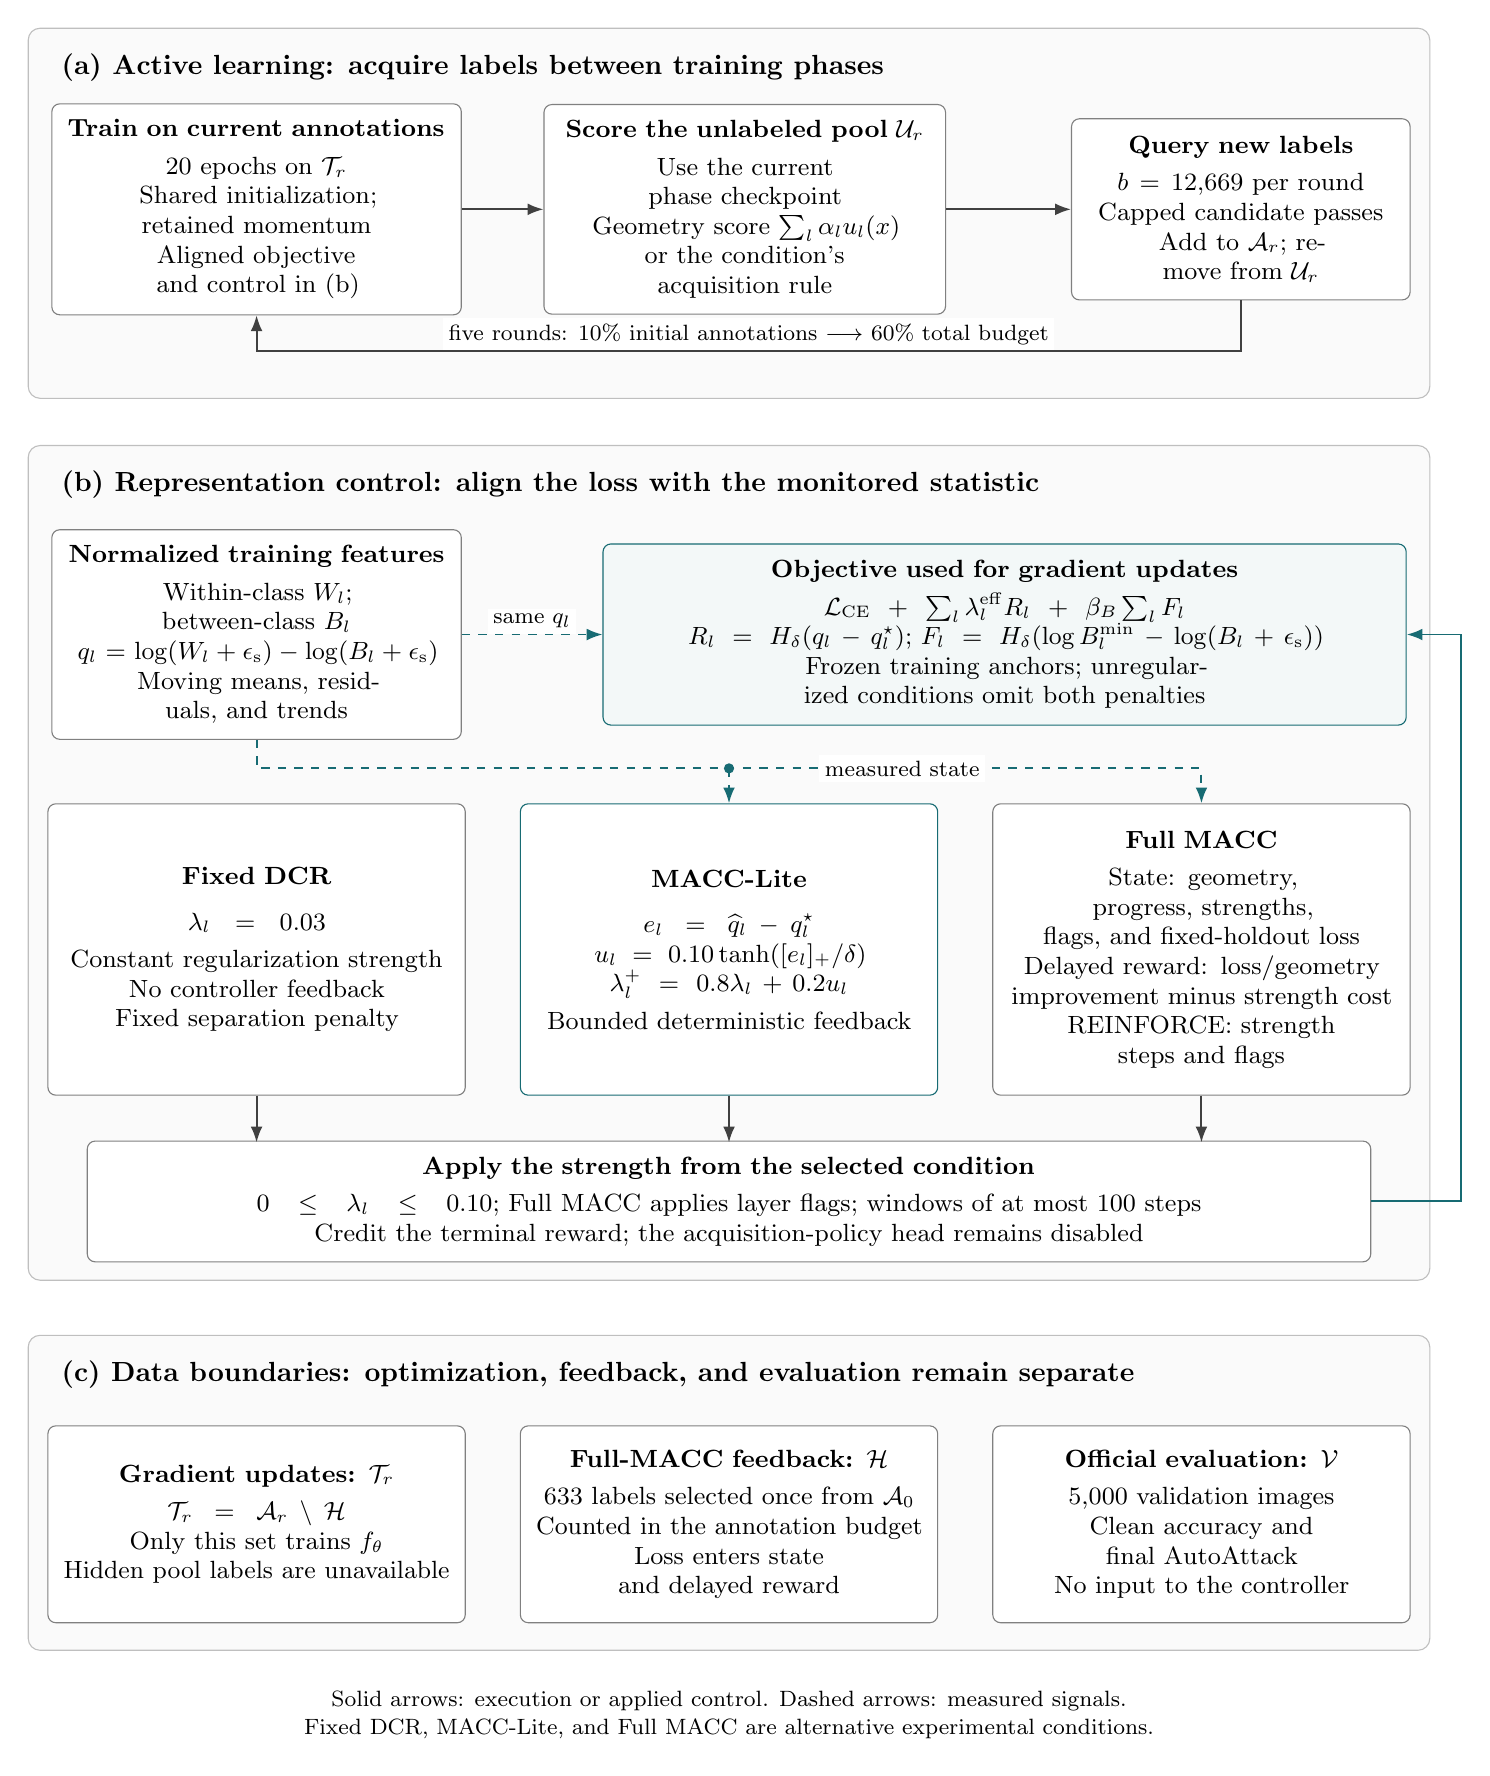
\begin{tikzpicture}[x=1mm,y=1mm,
 every node/.style={font=\fontsize{9}{10.7}\selectfont,align=center},
 box/.style={draw=black!50,rounded corners=1mm,fill=white,inner sep=2mm},
 panel/.style={draw=black!25,rounded corners=1.5mm,fill=black!2},
 head/.style={anchor=west,font=\fontsize{10}{12}\selectfont\bfseries},
 flow/.style={-{Latex[length=2mm]},line width=.7pt,draw=black!75},
 signal/.style={flow,dashed,draw=caenlaccent},
 label/.style={fill=white,inner sep=.7mm,font=\fontsize{8.5}{10}\selectfont}]

\draw[panel] (0,0) rectangle (178,-47);
\node[head] at (3,-5) {(a) Active learning: acquire labels between training phases};
\node[box,text width=48mm,minimum height=23mm] (train) at (29,-23) {
 \textbf{Train on current annotations}\\[1mm]
 20 epochs on $\mathcal T_r$\\
 Shared initialization; retained momentum\\
 Aligned objective and control in (b)};
\node[box,text width=47mm,minimum height=23mm] (acquire) at (91,-23) {
 \textbf{Score the unlabeled pool $\mathcal U_r$}\\[1mm]
 Use the current phase checkpoint\\
 Geometry score $\sum_l\alpha_lu_l(x)$\\
 or the condition's acquisition rule};
\node[box,text width=39mm,minimum height=23mm] (query) at (154,-23) {
 \textbf{Query new labels}\\[1mm]
 $b=12{,}669$ per round\\
 Capped candidate passes\\
 Add to $\mathcal A_r$; remove from $\mathcal U_r$};
\draw[flow] (train)--(acquire);
\draw[flow] (acquire)--(query);
\draw[flow] (query.south)--(154,-41)--node[label,above] {five rounds: 10\% initial annotations $\longrightarrow$ 60\% total budget} (29,-41)--(train.south);

\draw[panel] (0,-53) rectangle (178,-159);
\node[head] at (3,-58) {(b) Representation control: align the loss with the monitored statistic};
\node[box,text width=48mm,minimum height=23mm] (geometry) at (29,-77) {
 \textbf{Normalized training features}\\[1mm]
 Within-class $W_l$; between-class $B_l$\\
 $q_l=\log(W_l+\epss)-\log(B_l+\epss)$\\
 Moving means, residuals, and trends};
\node[box,draw=caenlaccent,fill=caenlaccent!5,text width=98mm,minimum height=23mm] (objective) at (124,-77) {
 \textbf{Objective used for gradient updates}\\[1mm]
 $\CE+\sum_l\lambda_l^{\mathrm{eff}}R_l+\beta_B\sum_l F_l$\\
 $R_l=H_\delta(q_l-q_l^\star)$; $F_l=H_\delta(\log B_l^{\min}-\log(B_l+\epss))$\\
 Frozen training anchors; unregularized conditions omit both penalties};
\draw[signal] (geometry)--node[label,above] {same $q_l$} (objective);

\node[box,text width=49mm,minimum height=37mm] (fixed) at (29,-117) {
 \textbf{Fixed DCR}\\[2mm]
 $\lambda_l=0.03$\\[1mm]
 Constant regularization strength\\
 No controller feedback\\
 Fixed separation penalty};
\node[box,draw=caenlaccent,text width=49mm,minimum height=37mm] (lite) at (89,-117) {
 \textbf{MACC-Lite}\\[2mm]
 $e_l=\widehat q_l-q_l^\star$\\
 $u_l=0.10\tanh([e_l]_+/\delta)$\\
 $\lambda_l^+=0.8\lambda_l+0.2u_l$\\[1mm]
 Bounded deterministic feedback};
\node[box,text width=49mm,minimum height=37mm] (full) at (149,-117) {
 \textbf{Full MACC}\\[1mm]
 State: geometry, progress, strengths,\\
 flags, and fixed-holdout loss\\
 Delayed reward: loss/geometry\\
 improvement minus strength cost\\
 REINFORCE: strength steps and flags};
\draw[signal] (geometry.south)--(29,-94)--(149,-94)--(full.north);
\draw[signal] (89,-94)--(lite.north);
\fill[caenlaccent] (89,-94) circle (.65mm);
\node[label] at (111,-94) {measured state};
\node[box,text width=159mm,minimum height=13mm] (strength) at (89,-149) {
 \textbf{Apply the strength from the selected condition}\\[1mm]
 $0\le\lambda_l\le0.10$; Full MACC applies layer flags; windows of at most 100 steps\\
 Credit the terminal reward; the acquisition-policy head remains disabled};
\draw[flow] (fixed.south)--(29,-140)--(29,-141.5);
\draw[flow] (lite.south)--(89,-141.5);
\draw[flow] (full.south)--(149,-140)--(149,-141.5);
\draw[flow,draw=caenlaccent] (strength.east)--(182,-149)--(182,-77)--(objective.east);

\draw[panel] (0,-166) rectangle (178,-206);
\node[head] at (3,-171) {(c) Data boundaries: optimization, feedback, and evaluation remain separate};
\node[box,text width=49mm,minimum height=25mm] at (29,-190) {
 \textbf{Gradient updates: $\mathcal T_r$}\\[1mm]
 $\mathcal T_r=\mathcal A_r\setminus\mathcal H$\\
 Only this set trains $f_\theta$\\
 Hidden pool labels are unavailable};
\node[box,text width=49mm,minimum height=25mm] at (89,-190) {
 \textbf{Full-MACC feedback: $\mathcal H$}\\[1mm]
 633 labels selected once from $\mathcal A_0$\\
 Counted in the annotation budget\\
 Loss enters state and delayed reward};
\node[box,text width=49mm,minimum height=25mm] at (149,-190) {
 \textbf{Official evaluation: $\mathcal V$}\\[1mm]
 5,000 validation images\\
 Clean accuracy and final AutoAttack\\
 No input to the controller};
\node[anchor=north,font=\fontsize{8.5}{10}\selectfont] at (89,-210) {
 Solid arrows: execution or applied control. Dashed arrows: measured signals.\\
 Fixed DCR, MACC-Lite, and Full MACC are alternative experimental conditions.};
\end{tikzpicture}%
}
\caption{The classification workflow of \model{}. (a) Acquisition expands the
annotated set between training phases. (b) The regularizer and adaptive
controllers use the same normalized scatter statistic, while the separation
safeguard penalizes insufficient between-class separation. Fixed strength, deterministic feedback, and learned feedback are
compared as alternatives. (c) The fixed holdout supplies Full-MACC feedback
without entering task-model gradient updates; official evaluation is separate.
Language, diffusion, and audio use the task-specific spectral formulations.
Prepared in TikZ with ChatGPT (OpenAI) assistance.}
\label{fig:detailed_workflow}\label{fig:framework_overview}
\end{figure*}



\subsection{Spectral formulation for language, diffusion, and audio}
\label{sec:spectral}

The other tasks use the separate spectral objective
\begin{equation}
 \mathcal L_{\mathrm{spec}}=
 \mathcal L_{\mathrm{task}}+
 \sum_{l\in\mathcal L}\lambda_l\|p_l-p_l^\star\|_2^2.
 \label{eq:spectral}
\end{equation}
This is spectrum matching, not a Frobenius penalty between
full covariance matrices and not the supervised scatter loss.

For a centered feature matrix $Z_l\in\R^{n_l\times d_l}$,
the implementation computes descending, nonnegative eigenvalues
of $Z_l^\top Z_l/n_l$, using the smaller Gram matrix
$Z_l Z_l^\top/n_l$ when appropriate. Let
$k_l=\min(k,d_l)$. The first $k_l$ eigenvalues are retained;
when fewer values are available, the vector is padded with zeros.
With this convention,
\begin{equation}
 p_{l,j}=
 \frac{\sigma_{l,j}}
 {\sum_{a=1}^{k_l}\sigma_{l,a}+\epsp},
 \quad j=1,\ldots,k_l,
 \qquad \epsp=10^{-8}.
 \label{eq:spectrum_normalization}
\end{equation}
The stabilizer means that the implemented vector is not exactly
unit mass when the retained spectral sum is very small.
For an exactly normalized nonzero spectrum $\pi$,
effective rank is $\exp(-\sum_j\pi_j\log\pi_j)$.
The monitor uses the full moving covariance spectrum rather than
the current truncated batch spectrum. Neither measurement is the
supervised trace ratio of Equation~\eqref{eq:trace_ratio}.

A rank-$r$ flat target places mass $1/r$ on the first $r$ entries.
The implementation restricts target rank to the available feature
and retained-spectrum dimensions and, when necessary, the centered
sample-rank bound $n_l-1$. Matching the eigenvalues does not specify
eigenvectors, class means, or an equiangular frame.

For diffusion, features are spatially pooled U-Net mid-block
activations and the task loss is noise-prediction mean squared error.
For audio, DCR acts on learned prefix embeddings and pooled
audio-token-encoder features; the task loss is next-token
cross-entropy. These experiments evaluate spectral regularization
without learned label acquisition.


\section{Supporting analysis}\label{sec:theory}

The analysis concerns the measured geometry, the effect of an isolated
aligned gradient, coefficient bounds, and additional conditions
connecting geometry to prediction. These are supporting
characterizations, not global optimization, generalization, or
input-space robustness guarantees for the training system.

\begin{proposition}[Scatter decomposition and invariance]
\label{prop:scatter}
For equal class weights and positive class counts, define
$T_l=K^{-1}\sum_c n_c^{-1}
\sum_{i:y_i=c}\|h_{i,l}-\bar\mu_l\|_2^2$.
Then $T_l=W_l+B_l$. Under
Equation~\eqref{eq:normalized_features}, $0\le T_l\le1$.
The three moments and $q_l$ are invariant under a common orthogonal
transformation. Away from the norm floor, they are invariant under
common positive rescaling of the raw features.
\end{proposition}
\begin{proof}
Expand
$h_{i,l}-\bar\mu_l=(h_{i,l}-\mu_{c,l})
+(\mu_{c,l}-\bar\mu_l)$.
The cross term vanishes within each class. Averaging gives
$T_l=W_l+B_l$. Moreover,
\[
 T_l=
 \frac1K\sum_c\frac1{n_c}\sum_{i:y_i=c}\|h_{i,l}\|_2^2
 -\|\bar\mu_l\|_2^2\le1.
\]
Orthogonal transformations preserve norms and inner products.
Normalization cancels a common positive scale when neither
representation activates the norm floor.
\end{proof}

\begin{lemma}[Quadratic deviation is not covariance trace]
\label{lem:mahalanobis}
Let $Z$ have mean $\mu$ and covariance $\Sigma$, and let $A$ be
a fixed symmetric matrix. If second moments exist,
\begin{equation}
 \E[(Z-\mu)^\top A(Z-\mu)]=\tr(A\Sigma).
 \label{eq:quadratic_expectation}
\end{equation}
Euclidean squared deviation therefore has expectation
$\tr(\Sigma)$, while squared Mahalanobis deviation with
$A=\Sigma^{-1}$ has expectation $d$ when $\Sigma$ is nonsingular.
With $(\Sigma+\epsilon I)^{-1}$, $\epsilon>0$, the expectation
is $\sum_j\sigma_j/(\sigma_j+\epsilon)$ rather than $\tr(\Sigma)$.
\end{lemma}
\begin{proof}
Write the quadratic form as
$\tr(A(Z-\mu)(Z-\mu)^\top)$ and exchange expectation with the
finite-dimensional trace. Diagonalizing $\Sigma$ gives the
special cases.
\end{proof}
The identity does not establish that a high Mahalanobis score is an
optimal acquisition choice. If $A$ is estimated from the same random
sample, the fixed-matrix argument requires conditioning or further
analysis.

\begin{proposition}[Direct local alignment]\label{prop:local}
Fix a measurement batch, a layer, and a positive residual
$g(\theta)=q_l(\theta)-q_l^\star$. Suppose $g$ has an
$L_g$-Lipschitz gradient, with $L_g>0$, on a neighborhood
containing the step. For $\eta,\lambda\ge0$ and
$a=H_\delta'(g(\theta))\in[0,1]$, the isolated step
$\theta'=\theta-\eta\lambda a\nabla g(\theta)$ satisfies
\begin{align}
 g(\theta')\le g(\theta)
 -\eta\lambda a
 \left(1-\frac{L_g\eta\lambda a}{2}\right)
 \|\nabla g(\theta)\|_2^2.
 \label{eq:alignment_bound}
\end{align}
The bound is nonincreasing when
$0\le\eta\lambda a\le2/L_g$.
\end{proposition}
\begin{proof}
Apply
$g(\theta+v)\le g(\theta)+\nabla g(\theta)^\top v+
(L_g/2)\|v\|_2^2$
with $v=-\eta\lambda a\nabla g(\theta)$.
\end{proof}
This result concerns one isolated loss component on a fixed batch.
It does not imply monotone scatter reduction under the combined
loss, momentum, augmentation, changing minibatches, or moving
observations. It also does not establish that explicit
objective--feedback alignment is necessary for useful control.

\begin{proposition}[Bounded feedback coefficients]\label{prop:bounded}
If $0\le\lambda_{l,0}\le\lambda_{\max}$ and $0<\rho\le1$,
Equation~\eqref{eq:lite} keeps every coefficient in that interval.
For a fixed residual, so that $u_{l,t}=u_l$,
\begin{equation}
 \lambda_{l,t}-u_l=(1-\rho)^t(\lambda_{l,0}-u_l).
\end{equation}
\end{proposition}
\begin{proof}
The desired coefficient lies in $[0,\lambda_{\max}]$.
Each update is a convex combination of that value and the previous
coefficient. For a fixed input, subtract $u_l$ and iterate.
\end{proof}
This establishes coefficient bounds and a fixed-input response.
It does not establish stability of the coupled network--controller
system. Full MACC's projection supplies coefficient bounds but
not this deterministic response formula.

\begin{proposition}[Conditional nearest-centroid error bound]
\label{prop:centroid}
Let population class means $\mu_c$ have minimum pairwise distance
$d_{\min}>0$, and assume equal class probabilities. A
nearest-centroid classifier has error probability at most
\begin{equation}
 \min\{1,4W/d_{\min}^2\},
 \qquad
 W=\frac1C\sum_c
 \E[\|H-\mu_c\|_2^2\mid Y=c].
\end{equation}
\end{proposition}
\begin{proof}
A feature within distance $d_{\min}/2$ of its true mean is
closer to that mean than to any other. An error therefore requires
$\|H-\mu_Y\|_2^2\ge d_{\min}^2/4$.
Apply Markov's inequality and average over classes.
\end{proof}
This is a population result for a particular classifier.
The trained softmax classifier need not use the nearest-centroid
rule; a batch ratio is not a population bound; and aggregate
$B_l>0$ does not ensure separation of every pair.
Reducing $q_l$ alone therefore need not reduce this bound.

\paragraph{Input-space robustness.}
Let $m_{y,j}(x)=f_y(x)-f_j(x)$.
If every margin is $L_{y,j}$-Lipschitz on the relevant
$L_\infty$ ball, then
$m_{y,j}(x)>\epsilon L_{y,j}$ for all $j\ne y$ is sufficient
to preserve the correct class throughout that ball, because
\[
 m_{y,j}(x+v)\ge m_{y,j}(x)-L_{y,j}\|v\|_\infty.
\]
Neither DCR formulation bounds those Lipschitz constants.
Geometry and empirical robustness are therefore measured separately.


\section{Experimental design}\label{sec:experiments}

\subsection{Study sequence and evidence separation}\label{sec:study_sequence}

Engineering checks verify implementation behavior and are not counted
as predictive-performance experiments. The original ImageNet-100
spectral pilot uses seeds 601 and 602. Saved-checkpoint attack
diagnostics and a bounded aligned-objective development screen
precede the final seeds 801--806. The aligned and spectral
development protocols also differ in sampling, BatchNorm treatment,
and integration choices; their absolute accuracies cannot isolate
the effect of changing DCR.

The initial ImageNet-100 comparison evaluated nine conditions across six
paired seeds. After reviewing those results, we evaluated two additional
conditions: entropy acquisition with aligned DCR and MACC-Lite, and a
matched-protocol UHerding-Margin comparator. Each used the original six
seed-specific initializations, targets, splits, annotation budgets, and
evaluation endpoint. Their comparison lists were fixed before the
additional runs, and their statistical families are reported separately.
A third follow-up added entropy with fixed aligned DCR, retaining the
same per-seed initial model and optimizer, splits, targets, floor penalty,
acquisition protocol, and optimization schedule. Its two contrasts were
declared before the new fixed-condition outcomes were inspected, after
the entropy and Lite outcomes were already known. This later control
adds six runs and 30 phases; it is not fresh-seed confirmation.
Throughout this paper, a \emph{condition} is a method configuration, a
\emph{run} is one condition under one seed, and a \emph{phase} is one
acquisition/training stage within a run. The resulting classification
record comprises 72 method--seed runs and 360 post-initialization phases
across 12 conditions; the number of independent paired seeds remains six.

C4 uses six separate training seeds and an additional unused-shard
evaluation of the same saved checkpoints.
Diffusion development uses seeds 1001 and 1002, followed by
confirmation seeds 1101--1106. Audio development uses seeds
1201 and 1202 for two epochs per condition; confirmation uses
seeds 1301--1306 for ten epochs. Confirmation starts from the
original pretrained assets and new seed-specific task components,
not development-final checkpoints. Only audio confirmation
evaluates caption-model predictions on the retained official test
split. Development results are not pooled into confirmation inference.

\subsection{ImageNet-100 data and label accounting}

We use the fixed 100-class subset associated with Contrastive
Multiview Coding~\cite{tian2020cmc}, drawn from
ImageNet~\cite{deng2009imagenet}.
It contains 126,689 training images and 5,000 validation images,
with 50 validation images per class. Original image bytes and
dimensions are retained. A manifest records class mappings, source
revision, paths, and SHA-256 values, which are checked before
execution. The evaluated benchmark is ImageNet-100, not ImageNet-1K.

Stratified sampling supplies 12,669 initial annotations per seed.
The controller holdout contains 633 of these, leaving 12,036
gradient-training images. Five rounds each acquire 12,669
additional examples. Annotation totals are 12,669, 25,338, 38,007,
50,676, 63,345, and 76,014. The final gradient-training set
contains 75,381 images. The final annotation fraction is
approximately $60.0005\%$, reported as 60\%.
Holdout labels are included in every method's annotation cost.
Pool labels are consulted only after selection.

\subsection{Classification optimization and matching}

The backbone is a randomly initialized ResNet-50 with a 100-class
head~\cite{he2016deep}. Each seed has one shared 40-nominal-epoch
cross-entropy initialization, reused by the original methods and
later matched conditions.
A physical minibatch contains 16 uniformly selected represented
classes and eight distinct acquired examples per class.
A nominal epoch has $\lceil|\mathcal T_r|/128\rceil$ sampled
minibatches rather than a permutation pass through the labeled set.

Training uses random resized $224\times224$ crops and horizontal
flips. Scoring, feedback, and evaluation resize the shorter side to
256 and take a 224-pixel center crop. ImageNet normalization is
inside the model, so attacks act in pixel space.
Augmentation and sampling streams are keyed by seed, phase, step,
and example index. Common random-number conventions do not make
sampled images identical once acquired sets differ.

Optimization uses SGD with momentum 0.9, Nesterov acceleration,
and weight decay $10^{-4}$ on multidimensional parameters.
One-dimensional parameters receive no decay.
Parameters remain FP32 with BF16 autocast, and gradients are
clipped at norm 5. Initialization uses learning rate 0.05,
three nominal warm-up epochs, and cosine decay.
Each subsequent 20-epoch phase starts at rate 0.025 with one
warm-up epoch and cosine decay; momentum is retained.
BatchNorm running statistics are updated during initialization
and frozen afterward; affine parameters remain trainable.

The five acquired-label phases contain 3,880, 5,840, 7,820,
9,800, and 11,780 optimizer steps.
Initialization contains 3,800 steps.
Each conceptual condition run therefore includes 42,920 steps and
5,493,760 sampled example presentations. Initialization is executed
once per seed and allocated once per conceptual condition when
reporting comparable costs.

\begin{table*}[pos=tbp]
\caption{Original frozen ImageNet-100 matrix. All nine conditions use
seeds 801--806 and the same 10--60\% annotation schedule.
``None'' disables both aligned penalties; all conditions record geometry.
The three follow-up conditions are reported separately.}
\label{tab:baselines}
\centering\small
\begin{tabularx}{\textwidth}{@{}p{0.30\textwidth}p{0.25\textwidth}Y@{}}
\toprule
Condition & Acquisition & Representation control \\
\midrule
Random & Uniform random selection & None \\
Entropy & Highest predictive entropy & None \\
BADGE & Exact factorized weight-gradient distances &
None; independent implementation, bias excluded \\
Noise Stability & Perturbed-output deviations with greedy coverage &
None; five noise draws, independent implementation \\
\model{} acquisition only &
Predicted-class diagonal Mahalanobis score & None \\
Random + aligned fixed DCR & Uniform random selection &
Aligned objective, $\lambda_l=0.03$ \\
\model{} + aligned fixed DCR & Mahalanobis score &
Aligned objective, $\lambda_l=0.03$ \\
\model{} + aligned MACC-Lite & Mahalanobis score &
Bounded, smoothed coefficient feedback \\
\model{} + aligned Full MACC & Mahalanobis score &
Learned coefficient increments and activation flags \\
\bottomrule
\end{tabularx}
\end{table*}

\subsection{Baselines and acquisition cost}

Table~\ref{tab:baselines} separates acquisition, regularization,
and adaptation.
BADGE uses exact factorized last-linear-layer weight-gradient
inner products rather than the pilot's random projection;
bias terms are excluded.
Noise Stability uses five globally normalized Gaussian
perturbations of the trainable parameter vector at relative
scale 0.001, normalized softmax-output deviations, concatenation
without projection, and greedy farthest-first selection.
Model parameters and buffers are restored after noisy forwards.

Nonrandom methods cache required pool outputs at the current
checkpoint. Mahalanobis acquisition additionally estimates class
statistics from acquired examples.
Equal annotation budgets and pass sizes do not equalize
acquisition time, especially for Noise Stability.
Random plus aligned fixed DCR tests whether the objective
contributes without geometric acquisition.
The final matrix has no new full-label reference; the pilot's
different-budget supervised reference is not mixed into the
matched final comparison.

\subsection{UHerding-Margin: matched-protocol implementation}
\label{sec:uherding_setup}

The recent comparator implements the uncertainty-weighted coverage
mechanism of Uncertainty Herding~\cite{bae2025uncertainty},
as \texttt{uherding\_margin\_initial\_r50}.
Each seed's shared-initial supervised ResNet-50 supplies
unit-normalized layer4 features $g_i$, cached for the full
training pool and fixed across rounds.
This differs from a separately pretrained self-supervised
representation. The task classifier continues under the
common warm-start schedule.

Before acquisition, temperature $T$ minimizes 15-bin ECE over
81 logarithmically spaced values in $[0.1,10]$ using the
budgeted 633-image holdout.
Temperature-scaled probabilities define
$\omega_i=1-(p_{i,(1)}-p_{i,(2)})$.
The bandwidth $\sigma$ is the smallest positive Euclidean
distance between fixed features of currently annotated examples,
including held-out annotations. Squared distances at most
$10^{-12}$ are numerical zero.
The kernel is
$k_\sigma(g_i,g_j)=\exp(-\|g_i-g_j\|_2^2/\sigma^2)$.

For candidate pass $P$, greedy selection maximizes
\begin{equation}
 G_P(j\mid\mathcal C)=
 \sum_{i\in P}\omega_i
 \left[
 k_\sigma(g_i,g_j)-
 \max_{a\in\mathcal C}k_\sigma(g_i,g_a)
 \right]_+,
 \label{eq:uherding_gain}
\end{equation}
where $\mathcal C$ contains annotated centers and examples
already selected in the round.
The 10,000-candidate and 10\%-per-pass convention is retained
until 12,669 new examples are acquired.
Distances, kernels, and gains use float64.
Lazy greedy is checked against exhaustive greedy on
deterministic CPU and CUDA fixtures.

No DCR is applied. Initializations, optimizer states, label
accounting, balanced batches, post-initialization BatchNorm
treatment, and the final attack endpoint match the task protocol.
Feature extraction, acquisition including calibration, and
training are timed separately.
This comparison evaluates the disclosed adaptation, not the
original authors' representation, unrestricted selection domain,
or published benchmark scores.

\subsection{Classification evaluation and statistical analysis}
\label{sec:statistics}

Every completed phase is evaluated on all 5,000 official
validation images in full precision.
Reported outcomes include pooled cross-entropy, top-1 and top-5
accuracy, 15-bin ECE, and equal-class normalized moments.
The selected checkpoint is the final scheduled checkpoint,
not the best validation epoch.
Logits, predictions, labels, and compact class-moment sufficient
statistics are retained.

The final checkpoint receives standard
AutoAttack~\cite{croce2020autoattack} at $L_\infty$ radius $8/255$
on all 5,000 images.
Its components are APGD-CE, targeted APGD, targeted FAB,
and Square Attack, without shortened prescribed iterations.
Attack minibatches contain 64 images; restartable storage chunks
contain 256. Pixel bounds, perturbation norms, and survival masks
are recorded. No adversarial training is used.
A compatibility repair changed \texttt{view} to \texttt{reshape}
in the library's zero-gradient diagnostic, retaining the diagnostic,
attack configuration, and completed training.

The paired experimental units are six seeds, conditional on the
fixed dataset and protocol.
Seven contrasts are specified separately for final clean and
robust accuracy. For target-minus-reference differences $d_i$,
the individual paired-$t$ interval is
\[
 \bar d\pm t_{0.975,5}\frac{s_d}{\sqrt6}.
\]
Both paired-$t$ tests and enumeration of all $2^6$ sign flips
are retained. Holm correction~\cite{holm1979} is applied within
each declared endpoint and test family.
Intervals are individual, unadjusted intervals, not simultaneous
confidence bands. The paired-$t$ analysis relies on its
distributional approximation for the differences. Interpreting
sign-flip enumeration as an exact null test requires the
corresponding sign-exchangeability or symmetry assumption;
enumeration alone does not make it assumption-free.

\paragraph{Resolution of the six-seed exact tests.}
\label{sec:exact_resolution}
For the two-sided absolute-mean statistic, an observed sign pattern
and its global negation are both at least as extreme as the observed
absolute mean. Therefore
\begin{equation}
 p_{\mathrm{exact}}\ge\frac{2}{2^6}=0.03125.
 \label{eq:exact_resolution}
\end{equation}
In a Holm family of $m\ge2$ comparisons at $\alpha=0.05$,
the first rejection threshold is
$0.05/m\le0.025$.
Consequently, no rejection is attainable under these six-seed,
two-sided, Holm-adjusted exact tests.
A smallest raw value of 0.03125 expresses the strongest attainable
sign-flip evidence at this resolution, not adjusted significance.
All declared tests and adjustments are reported with this resolution
limit; it is not evidence that their underlying effects are absent.

The entropy-plus-Lite, UHerding, and entropy-plus-fixed follow-ups each
use a separate two-contrast clean-accuracy family, specified before the
respective additional runs but after earlier outcomes were available.
For UHerding, the contrasts are UHerding minus entropy and
entropy-plus-Lite minus UHerding. For the fixed-control follow-up, they
are entropy-plus-fixed minus entropy and entropy-plus-Lite minus
entropy-plus-fixed. New fixed-condition robustness is descriptive;
the original robustness family is unchanged.
These within-family corrections do not provide one family-wise
error guarantee for the full sequential research programme.
Geometry, calibration, top-5 accuracy, and intermediate budgets
are descriptive secondary outcomes.

\subsection{Cross-task experimental protocols}\label{sec:cross_protocols}
These protocols concern Equation~\eqref{eq:spectral}. The fixed, Lite,
and Full names identify task-specific implementations; the aligned
classification loss is not used in these studies.
\begin{table*}[pos=tbp]
\caption{Task-specific regularization and feedback conventions.
``Lite'' and ``Full'' denote different task-specific implementations,
not an unchanged controller transferred across all tasks.
Task protocols provide the remaining settings.}
\label{tab:control_variants}
\centering\small
\begin{tabularx}{\textwidth}{@{}p{0.17\textwidth}YYY@{}}
\toprule
Task & Loss and observed statistic & Fixed/adaptive coefficients &
Update convention \\
\midrule
ImageNet-100 classification &
Aligned normalized within/between log ratio; fixed separation safeguard &
Fixed $0.03$; adaptive initialization $0.03$; bounds $[0,0.10]$ &
Aligned Lite uses the leaky rule; Full uses the aligned reward;
windows of at most 100 steps and phase-boundary handling \\
GPT-2/C4 &
Spectral loss with $k=128$, ranks 16 and 4 at h6/h12;
separate covariance-spectrum feedback &
Fixed $0.01$; adaptive initialization $0.005$;
bounds $[0,0.08]$ &
Spectral control every 25 steps;
Lite step size $0.002$ and deadband $0.1$ \\
CIFAR-10 diffusion &
Spectral loss with $k=64$, rank-16 target;
full EMA-covariance monitor &
Fixed $0.01$; adaptive initialization $0.01$;
bounds $[0,0.05]$ &
Spectral control every 50 steps;
Lite step size $0.001$ and deadband $0.1$ \\
AudioCaps captioning &
Spectral loss with $k=64$, rank-16 targets at prefix/encoder;
different sample axes and zero padding &
Fixed $0.01$; adaptive initialization $0.01$;
bounds $[0,0.05]$ &
Spectral control every 50 steps and final step;
terminal reward credited without an unused next action \\
\bottomrule
\end{tabularx}
\end{table*}

\subsubsection{Language modeling on C4}
\label{sec:c4_setup}

Pretrained GPT-2~\cite{radford2019gpt2}, with 124,439,808 parameters,
is fine-tuned on a deterministic C4 subset~\cite{raffel2020}.
Each of seeds 301--306 processes 99,999,744 tokens in 12,207
steps, with sequence length 1,024 and eight sequences per step.
Baseline, fixed spectral DCR, spectral MACC-Lite, and spectral
Full MACC share the budget and training configuration.
The spectral implementation monitors h6 and h12 with target
ranks 16 and 4, retained spectrum size 128, and a 2,048-token
DCR subsample. Fixed strength is 0.01.

Training uses the first English C4 training shard, with the first
validation shard used for feedback and development
(Appendix~\ref{app:provenance}). All four conditions therefore
evaluate the same single-shard training distribution.
The original reporting set has 1,889 validation sequences, with
64 additional sequences reserved for controller feedback.

After checkpoint selection and training were frozen, all 24
checkpoints were evaluated on validation shard 00002,
which had not been used for local training, feedback,
or configuration development.
Each checkpoint makes 1,999,872 next-token predictions.
NLL and accuracy are pooled over tokens; ECE is computed from
pooled confidence-bin statistics.
Perplexity is the exponential of NLL, not an independent endpoint.
``Untouched'' concerns local study use, not verified absence of
GPT-2 pretraining overlap.

Optimization uses learning rate $5\times10^{-5}$,
weight decay 0.01, and 200 warm-up steps.
AdamW has $\beta_1=0.9$, $\beta_2=0.95$;
one-dimensional, bias, and normalization parameters are exempt
from decay. Norm-1 clipping and linear warm-up followed by
cosine decay toward 10\% of the base rate are used.
Parameters remain FP32 with BF16 CUDA autocast.

Spectral controllers operate every 25 steps.
Both adaptive methods initialize their coefficients at 0.005
within $[0,0.08]$.
Spectral Lite uses step size 0.002 and deadband 0.1.
Full MACC uses two 128-unit hidden
layers, policy learning rate $3\times10^{-4}$,
exploration probability $0.15$ decreasing to $0.02$,
reward-baseline weight 0.1, and entropy coefficient 0.001.
Its coefficient increments are
$\{-0.005,-0.0025,0,0.0025,0.005\}$.
Its language-specific reward settings include validation-delta
scale 5.0, value-delta clip 0.1, target-deviation weight 0.005,
and zero query penalty.
These settings are not replaced by the later diffusion/audio
or aligned-classification controller settings.

The unused-shard evaluator compares fixed DCR, Lite, and Full separately
with baseline, giving three contrasts per endpoint. It reports individual
paired-$t$ intervals, raw paired-$t$ and exact sign-flip values, and Holm
adjustment of the paired-$t$ values within each three-contrast family.
Holm adjustment is applied separately to the paired-$t$ and exact
values within each endpoint family. NLL is primary; perplexity is its
monotone transformation, while token accuracy and ECE remain secondary.


\subsubsection{CIFAR-10 diffusion}
\label{sec:diffusion_setup}

We fine-tune the 35,746,307-parameter pretrained
\path{google/ddpm-cifar10-32} U-Net with the noise-prediction
objective~\cite{ho2020denoising}.
Seeds 1101--1106 evaluate baseline fine-tuning, fixed spectral
DCR, spectral MACC-Lite, and spectral Full MACC.
The unchanged pretrained model is also sampled with each seed's
generation-noise stream. Those six references measure sampling
variation for one model, not six pretrained-model replications.

A fixed partition of the original 50,000 CIFAR-10 training
images~\cite{krizhevsky2009cifar}
supplies 45,000 fine-tuning images and 5,000 internal holdout
images. The holdout contains 256 controller images and
1,024 disjoint denoising-assessment images with fixed noise
and timesteps. These images may have been seen during
pretraining; the holdout is not pristine relative to the
pretrained model. Official test outcomes do not enter control
or checkpoint selection.

Each trained condition performs 10,000 updates with batch size
128, matched per-seed image order and noise streams,
horizontal flips, AdamW learning rate $2\times10^{-5}$,
zero weight decay, and norm-1 clipping.
Parameters are FP32 with BF16 autocast.
EMA weights use decay 0.9995.
The final scheduled checkpoint is retained independently of
performance. No active label acquisition occurs.

DCR uses 256-dimensional spatially pooled mid-block features
across timesteps 0--999, retained spectrum size 64,
and target rank 16.
The full EMA-covariance monitor uses decay 0.99 and cadence
50 steps. Fixed strength is 0.01.
Adaptive methods start at 0.01 within $[0,0.05]$.
For finite monitored rank $r_{\mathrm{eff},l,t}$, spectral Lite uses
\begin{align}
 e^{\mathrm{sp}}_{l,t}
 &=\left|\log\!\left(
 \frac{\max\{r_{\mathrm{eff},l,t},10^{-12}\}}{16}
 \right)\right|-0.1,\nonumber\\
 \lambda_{l,t+1}
 &=\Pi_{[0,0.05]}\!\left(\lambda_{l,t}
                +0.001e^{\mathrm{sp}}_{l,t}\right),
 \label{eq:spectral_lite_update}
\end{align}
where $\Pi_{[a,b]}(v)=\min\{b,\max\{a,v\}\}$.
The error is not replaced by its positive part: the coefficient
increases outside the log-rank deadband, decreases inside it, and
is unchanged at its boundary, subject to projection. Missing or
nonfinite rank observations leave the corresponding coefficient
unchanged. This accumulating projected rule differs from the leaky
classification rule in Equation~\eqref{eq:lite}.
% core/controllers.py, SHA-256
% 9e5fb0237e49643a9a2e8b24077a5b9f1cfd81487be298aa549d432a5345b88e.
% The diffusion source manifest pins this exact file; error() returns
% abs(log(max(rank,1e-12)/max(target,1e-12)))-deadband, then step()
% adds step_size*error and clips the coefficient. Target rank is 16.

Spectral Full MACC uses the retained two-layer 128-unit policy,
increments $\{-0.005,-0.0025,0,0.0025,0.005\}$,
activation flags, policy learning rate $3\times10^{-4}$,
exploration decreasing from 0.10 to 0.02, baseline weight 0.05,
and entropy coefficient 0.001.
Its reward combines the scaled held-out loss improvement
(scale 10, clipped to $[-2,2]$) and a
$-0.1|\log(r_{\mathrm{eff}}/16)|$ target-deviation term.
The query head is disabled, and uniformly explored actions
are excluded from on-policy gradient updates.
At termination, the pending action is credited without sampling
an unused next action.

Each final EMA model generates 50,000 uint8 images with
DDIM~\cite{song2021ddim}, 100 sampling steps, $\eta=0$,
and batches of 128. Noise streams are matched within a seed.
The primary endpoint is FID~\cite{heusel2017fid} against the
complete original 50,000-image training distribution, using
\texttt{torch-fidelity} 0.4.0.
KID~\cite{binkowski2018mmd} and Inception
score~\cite{salimans2016gan} are secondary.
A final EMA denoising assessment uses all 10,000 official test
images and fixed noise/timestep seed 541211.
Per-image errors are retained.

Four FID contrasts are frozen: baseline minus pretrained
reference and each regularized condition minus baseline.
Negative differences favor the target.
Paired-$t$ and all 64 sign flips are reported with separate
Holm correction across these four contrasts.
The exact-resolution limitation in
Section~\ref{sec:statistics} applies.
Development uses two different seeds, 2,000 updates,
and 5,000 generated samples; its absolute FID values are
not pooled with confirmation.

\subsubsection{AudioCaps captioning}
\label{sec:audio_setup}

The audio study uses original AudioCaps
annotations~\cite{kim2019audiocaps} and a documented
available-recording subset from
\path{OpenSound/AudioCaps}.
All 473 hosted Parquet shards were checked against published
digests. IDs, start times, and captions were matched to pinned
original annotations.
The retained counts are 44,466 training, 440 validation,
and 866 test clips, versus original inventories of
49,838, 495, and 975 unique clips.
Coverage is 89.22\%, 88.89\%, and 88.82\%.
Each retained validation/test clip has five references.

Preparation excludes recordings outside eight to twelve seconds,
one test identity with conflicting decoded variants,
and both members of a nonzero waveform duplicate spanning train
and test. Sources, variants, and exclusion records are preserved.
Four all-zero training waveforms remain flagged and retained.
Checks found no cross-split video IDs or exact nonzero waveform
duplicates, including after actual mono/resampling preprocessing.
These checks do not establish acoustic authenticity, absence
of near-duplicates, or equivalence to an official raw-audio
distribution. The mirror's provenance and licensing limitations
remain explicit; raw audio is not redistributed.

The frozen Audio Spectrogram Transformer
(AST)~\cite{gong2021ast} checkpoint
\path{MIT/ast-finetuned-audioset-10-10-0.4593}
supplies shared features.
Channels are averaged, resampled to 16 kHz, and limited to the
first 10.24 seconds for a single-window representation.
Original waveforms are not rewritten.
FP32 AST computation supplies 64 pooled patch tokens of
dimension 768, stored in FP16 and reused read-only.
The test features use the frozen backbone only.
AudioSet~\cite{gemmeke2017audioset} pretraining may include
underlying recordings, so no absence of pretraining overlap
is claimed.

The task model has a two-layer trainable audio-token encoder,
an eight-token learned prefix, and trainable pretrained GPT-2,
totaling 141,774,336 parameters.
Baseline, fixed spectral DCR, spectral Lite, and spectral Full
use matched accepted initial task weights, epoch permutations,
per-step dropout seeds, and optimizer budgets.
Seeds 1301--1306 start from original GPT-2 assets and new
seed-specific encoder/prefix parameters, not pilot-final weights.
The initialization recovery is documented in
Appendix~\ref{app:provenance}.

AdamW uses encoder/prefix rate $10^{-4}$, decoder rate
$5\times10^{-5}$, decay 0.01, and norm-1 clipping.
Parameters remain FP32 with BF16 autocast.
Each epoch permutes 44,466 training pairs and uses
1,389 batches of 32, dropping the last 18 pairs.
A new deterministic permutation is used every epoch.
Each of the 24 runs performs ten epochs, or 13,890 updates.

For zero-based optimizer-step index $s=0,\ldots,S-1$, with
$S=13{,}890$ and $w=100$ warm-up steps, every parameter group's
base rate $\eta_{g,0}$ is multiplied by
\begin{equation}
 a(s)=
 \begin{cases}
 (s+1)/w, & 0\le s<w,\\[2pt]
 \dfrac{1+\cos\!\bigl(\pi p(s)\bigr)}{2}, & w\le s,
 \end{cases}
 \label{eq:audio_lr_schedule}
\end{equation}
where $p(s)=\min\{1,(s-w)/(S-w)\}$ and
$\eta_g(s)=\eta_{g,0}a(s)$.
The schedule has terminal factor zero and no positive learning-rate
floor. Its zero endpoint is $s=S$; the last executed update is
$s=S-1$, so its final applied factor is slightly above zero.
The final scheduled checkpoint is evaluated without best-epoch
selection or early stopping.
% audio/common.py::cosine_lr, SHA-256
% 432c7c003ebd598f34ff133e3ad9ae7ebd5ead490001612b3c8ba7b7fc9de5cc.
% audio/captioning.py, SHA-256
% 438c3284238702d31cebab8835d1f87242c5fae20d7eea969cb1011797ba7281,
% calls cosine_lr(self.step,self.total_steps,1.0,warmup) before each
% optimizer update. The confirmation wrapper retains this training loop.
% These two files are pinned in the confirmation engine's source manifest.

\paragraph{Spectral sample axes and rank.}
The prefix representation reshapes eight embeddings per clip
into $32\times8=256$ vectors of dimension 768.
The pooled encoder representation has 32 vectors of dimension 768.
Thus their centered sample-rank bounds are 255 and 31,
respectively. The configured 64-entry spectrum is a storage
and truncation dimension, not a claim of 64 nonzero eigenvalues
for both representations. The encoder Gram spectrum is
zero-padded to 64 entries as in
Equation~\eqref{eq:spectrum_normalization}.
A rank-16 template is feasible for both full training batches.
The EMA-covariance monitor is distinct from either current-batch
spectrum and can have a larger effective rank.

Control operates every 50 steps and at the final step,
yielding 278 adaptive events.
The fixed coefficient is 0.01.
Adaptive coefficients start at 0.01 within $[0,0.05]$.
Spectral Lite uses Equation~\eqref{eq:spectral_lite_update} at both
monitored layers, with step size 0.001, deadband 0.1, and target rank 16.
Full retains the diffusion spectral-policy settings, replacing
denoising feedback loss with caption loss on the audio holdout.
Its terminal action is credited without an unused next action,
and the acquisition head is disabled.

The first 64 validation IDs in frozen manifest order provide
controller feedback; the remaining 376 provide development
assessment. Neither is used for task-model gradient updates.
Final confirmation checkpoints evaluate all 866 retained test
recordings.
Beam size is three, decoding batch size is 32, and at most
30 new tokens are generated.

The primary endpoint is CIDEr-D~\cite{vedantam2015cider}
from the retained \texttt{pycocoevalcap}/PTB path.
BLEU-1--4~\cite{papineni2002bleu},
ROUGE-L~\cite{lin2004rouge},
METEOR~\cite{denkowski2014meteor},
SPICE~\cite{anderson2016spice},
SPIDEr~\cite{liu2017spider}, and pooled token NLL are
secondary outcomes.
SPIDEr combines CIDEr-D and SPICE on their recorded scales.
NLL is weighted by actual next-token target counts.
A separate development diagnostic mismatches audio and captions
deterministically without training updates.

The three primary CIDEr-D contrasts compare fixed, Lite,
and Full with baseline.
Positive differences favor the regularized condition.
Both paired-$t$ and all 64 sign flips are retained with
separate Holm corrections across these three comparisons
and individual unadjusted intervals.
Secondary outcomes do not replace the primary endpoint.
The six paired seeds remain the experimental units;
repeated evaluation of 866 clips does not create extra
training replications.


\subsection{Execution environment and reproducibility}

Experiments run sequentially on an IBM Cloud instance with one
NVIDIA L40S GPU, PyTorch 2.6.0, torchvision 0.21.0,
CUDA runtime 12.4, and Python 3.11.7.
Datasets and checkpoints reside on persistent storage.
Protocols, source hashes, splits, acquisitions, controller records,
summaries, and attack-chunk digests are retained.
Integrity checks establish consistency of recorded artifacts,
not third-party replication of GPU execution.


\subsection{Computational assistance and figure preparation}
\label{sec:computational_assistance}
ChatGPT (OpenAI) assisted with experimental-software development and
review, saved-result analysis, mathematical exposition, reference
checking, and LaTeX/TikZ/Matplotlib preparation. Numerical figures are
compiled from recorded measurements or explicitly stated statistical
summaries; schematic figures describe the implemented workflow.
Numerical outputs are derived from the recorded experiments and
reproducible calculations. The verification scope is described in
Appendix~\ref{app:provenance}.

\clearpage
\onecolumn
\begin{multicols}{2}
\section{Results and analysis}\label{sec:results}

\subsection{ImageNet-100 comparison across matched seeds}

Table~\ref{tab:imagenet100_final} consolidates all 12 evaluated conditions.
Entropy acquisition with aligned DCR and MACC-Lite has the highest mean
clean accuracy, $73.360\pm0.208\%$, compared with
$71.463\pm0.320\%$ for entropy alone and $71.747\pm0.626\%$ for
UHerding-Margin. The later entropy-plus-fixed condition reaches
$72.263\pm0.381\%$. The table distinguishes the initial comparison from
the three follow-up conditions; their inferential families remain separate.
Within the initial nine-condition comparison, geometric acquisition with
aligned MACC-Lite attains $72.120\pm0.490\%$. Adding fixed aligned DCR to
geometric acquisition gives +0.850 percentage points, and replacing fixed
strength with Lite gives another +1.080 points. Both component differences
are positive in all six paired seeds.
\end{multicols}

\begin{placedtable}
\caption{All 12 ImageNet-100 conditions at 60\% annotations.
Values are mean $\pm$ sample SD over six paired seeds; clean and standard
AutoAttack accuracy use all 5,000 validation images. Study I denotes the
initial nine-condition comparison, A the later acquisition-rule ablation,
B the later UHerding comparison, and C the later entropy-plus-fixed
control. The table is descriptive: study-specific inferential families
remain separate. Bold identifies the highest observed
mean clean accuracy, not a universal superiority claim.}
\label{tab:imagenet100_final}
\centering\small
\begin{tabularx}{\textwidth}{@{}p{0.23\textwidth}c*{4}{>{\centering\arraybackslash}X}@{}}
\toprule
Condition & Study & Clean top-1 (\%) & AutoAttack $8/255$ (\%) &
Cross-entropy & ECE \\
\midrule
Random & I & $69.293\pm0.334$ & $0.013\pm0.010$ & $1.272712\pm0.021145$ & $0.094945\pm0.002917$ \\
Entropy & I & $71.463\pm0.320$ & $0.010\pm0.011$ & $1.150591\pm0.020293$ & $0.079698\pm0.003849$ \\
BADGE & I & $71.110\pm0.467$ & $0.003\pm0.008$ & $1.149581\pm0.007022$ & $0.077088\pm0.004058$ \\
Noise Stability & I & $71.023\pm0.249$ & $0.003\pm0.008$ & $1.162821\pm0.006167$ & $0.078703\pm0.002375$ \\
\model{} acquisition only & I & $70.190\pm0.240$ & $0.013\pm0.010$ & $1.210545\pm0.010404$ & $0.085552\pm0.004501$ \\
Random + aligned fixed DCR & I & $70.113\pm0.452$ & $0.017\pm0.008$ & $1.217939\pm0.021315$ & $0.085964\pm0.006228$ \\
\model{} + aligned fixed DCR & I & $71.040\pm0.427$ & $0.017\pm0.008$ & $1.155351\pm0.015230$ & $0.078428\pm0.003667$ \\
\model{} + aligned MACC-Lite & I & $72.120\pm0.490$ & $0.007\pm0.010$ & $1.078885\pm0.008014$ & $0.062948\pm0.004965$ \\
\model{} + aligned Full MACC & I & $70.803\pm0.318$ & $0.007\pm0.010$ & $1.171322\pm0.023746$ & $0.081639\pm0.004671$ \\
\midrule
Entropy + aligned MACC-Lite & A & $\mathbf{73.360\pm0.208}$ & $0.003\pm0.008$ & $1.028967\pm0.010101$ & $0.055426\pm0.001256$ \\
UHerding-Margin & B & $71.747\pm0.626$ & $0.007\pm0.010$ & $1.127922\pm0.021039$ & $0.073977\pm0.003294$ \\
Entropy + aligned fixed DCR & C & $72.263\pm0.381$ & $0.000\pm0.000$ & $1.092014\pm0.013386$ & $0.071037\pm0.004253$ \\
\bottomrule
\end{tabularx}
\end{placedtable}

\begin{multicols}{2}
Figure~\ref{fig:label_budget} shows the available per-phase clean-accuracy
measurements, separating acquisition rules from aligned regularization.
The budget trajectories are descriptive; the final 60\% endpoint remains
the basis of the declared clean-accuracy comparisons. The
entropy-plus-Lite and entropy-plus-fixed trajectories are shown
separately in Figure~\ref{fig:entropy_budget}, together with paired gains
over entropy. All displayed points are measured phase endpoints.
\end{multicols}

\begin{figure}[!tbp]
\centering
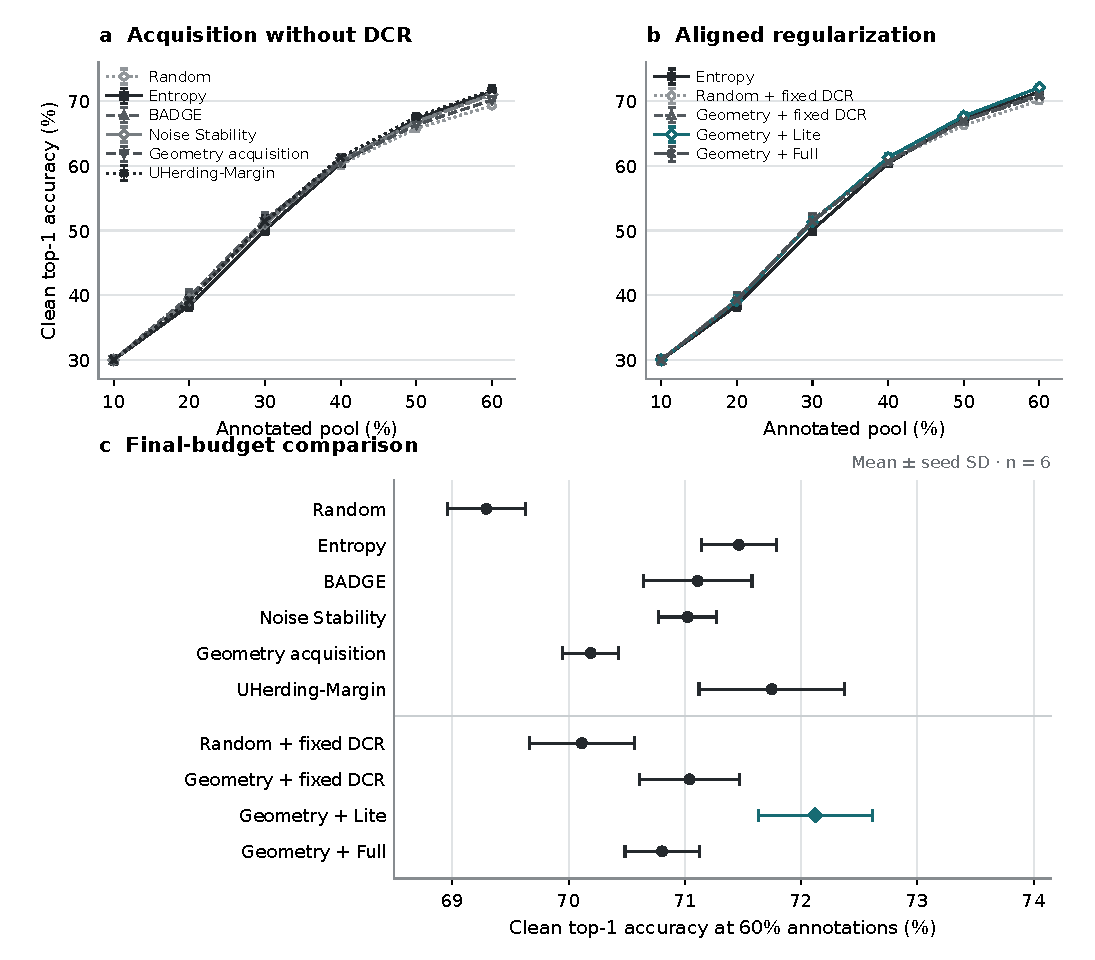
\includegraphics[width=\textwidth]{figures/figure2_budget.pdf}
\caption{Acquisition and aligned regularization under the common
ImageNet-100 protocol. Panels (a) and (b) show measured accuracy trajectories
on identical axes; panel (c) enlarges the final 60\% endpoint for the original
nine conditions and the UHerding-Margin follow-up. Markers and bars represent
six-seed means and sample SDs, not confidence intervals. All trajectories
start from the same 10\% checkpoint. Fixed, Lite, and Full denote aligned
DCR conditions; entropy regularization follow-ups appear in
Figure~\ref{fig:entropy_budget}. Connecting lines guide the eye, and no new
area-under-curve test or inferential family is introduced.}
\label{fig:label_budget}
\end{figure}

\begin{multicols}{2}
The two component contrasts pass the planned adjusted
paired-$t$ threshold.
Lite versus entropy does not: its raw paired-$t$ value
is 0.0466, but its adjusted value is 0.0931.
The individual interval narrowly excludes zero but is not a
simultaneous interval.
Figure~\ref{fig:paired_effects} preserves the original effects
and intervals.
The nonrejection of the adjusted exact tests must be interpreted
with their design-imposed resolution limit, not as an
independent demonstration that the effects are absent.

Acquisition alone improves over random by +0.897 points,
while random plus fixed aligned DCR improves by +0.820.
These comparisons show favorable directions for both components
within the declared regime. Acquisition alone remains below
entropy in mean accuracy.
The acquisition-rule ablation shows
that geometric acquisition is not necessary for the strongest
observed result. No equal-performance full-supervision
comparison establishes a 40\% annotation saving.
\end{multicols}

\begin{figure}[!tbp]
\centering
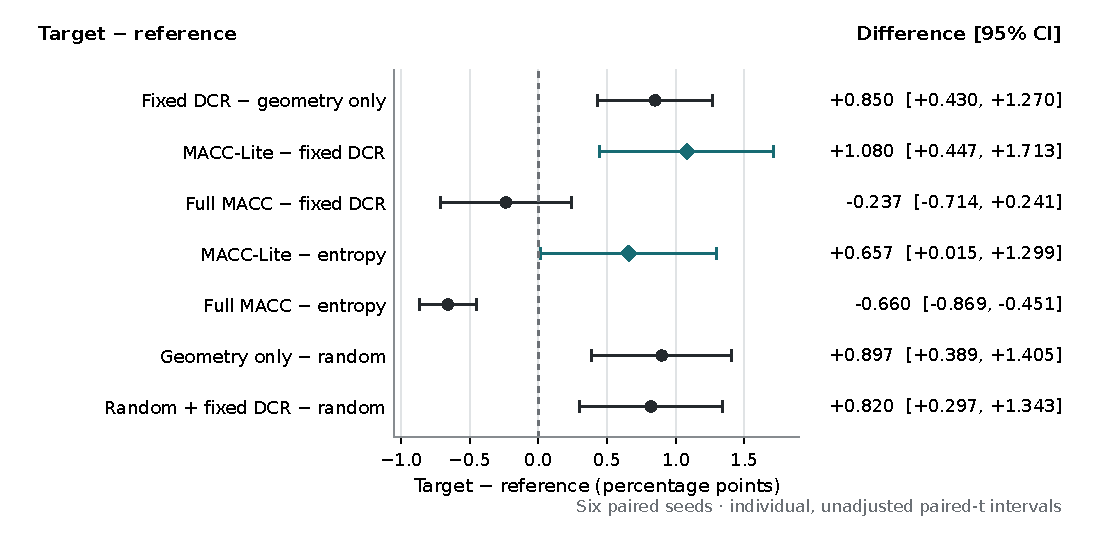
\includegraphics[width=\textwidth]{figures/figure3_effects.pdf}
\caption{All seven planned clean-accuracy contrasts in the original
nine-condition family. Points give the mean target-minus-reference
difference; bars and the numeric column give individual unadjusted 95\%
paired-$t$ intervals across six seeds. The dashed line denotes no difference.
Fixed DCR, MACC-Lite, and Full MACC use geometry acquisition unless random
acquisition is explicitly indicated. Accent color identifies Lite contrasts,
not statistical significance. Multiplicity-adjusted tests are reported in
Table~\ref{tab:planned_contrasts}; Lite versus entropy does not pass the
adjusted paired-$t$ threshold.}
\label{fig:paired_effects}
\end{figure}

\begin{placedtable}
\caption{All seven original clean-accuracy contrasts in percentage
points. Intervals are individual unadjusted 95\% paired-$t$
intervals. Each $p$-value column is separately Holm-adjusted
across seven contrasts. The exact tests have the resolution
limit described in Section~\ref{sec:statistics}.}
\label{tab:planned_contrasts}
\centering\small
\begin{tabularx}{\textwidth}{@{}Yrrrr@{}}
\toprule
Target minus reference & Difference (pp) & 95\% CI (pp) &
Adjusted $t$ $p$ & Adjusted exact $p$ \\
\midrule
Aligned fixed DCR $-$ acquisition only &
+0.850 & $[+0.430,+1.270]$ & 0.0208 & 0.2188 \\
Aligned MACC-Lite $-$ aligned fixed DCR &
+1.080 & $[+0.447,+1.713]$ & 0.0309 & 0.2188 \\
Aligned Full MACC $-$ aligned fixed DCR &
$-0.237$ & $[-0.714,+0.241]$ & 0.2589 & 0.2813 \\
Aligned MACC-Lite $-$ entropy &
+0.657 & $[+0.015,+1.299]$ & 0.0931 & 0.2188 \\
Aligned Full MACC $-$ entropy &
$-0.660$ & $[-0.869,-0.451]$ & 0.0032 & 0.2188 \\
Acquisition only $-$ random &
+0.897 & $[+0.389,+1.405]$ & 0.0309 & 0.2188 \\
Random + aligned fixed DCR $-$ random &
+0.820 & $[+0.297,+1.343]$ & 0.0309 & 0.2188 \\
\bottomrule
\end{tabularx}
\end{placedtable}

\begin{multicols}{2}
\subsection{Acquisition-rule ablation under aligned MACC-Lite}
\label{sec:entropy_lite}

The acquisition-rule condition replaces geometric acquisition with
entropy while retaining the aligned objective, Lite settings,
six shared initializations, annotation and feedback splits,
targets, and five 20-epoch phases.
Its first acquisition is checked against the original entropy
selection. Thirty additional phases and full-set final attacks
are completed. These are paired acquisition-rule runs,
not new independent seeds for the original matrix.

Entropy with aligned DCR and Lite reaches
$73.360\pm0.208\%$ and exceeds unregularized entropy and
geometry-plus-Lite in every seed.
Table~\ref{tab:entropy_lite_supplement} gives the paired comparisons;
Appendix~\ref{app:classification_details} provides the seed-level
outcomes (Table~\ref{tab:entropy_lite_seeds}).


The gain over entropy is +1.897 percentage points, with individual
95\% paired-$t$ interval $[+1.625,+2.169]$. The gain over geometry plus
Lite is +1.240 points, with interval $[+0.707,+1.773]$. Both comparisons
pass the acquisition-rule adjusted paired-$t$ analysis. Their raw exact value is 0.03125 and adjusted value
0.0625, consistent with the resolution limit.
The evidence supports the \emph{combined aligned-loss-and-Lite
treatment within entropy acquisition}.
That acquisition-rule study did not include a fixed-strength entropy
control. The later matched follow-up in Section~\ref{sec:entropy_fixed}
provides that comparison while preserving the acquisition-rule study's
original two-contrast family.

One image survives the attack for seed 802 and none for the
other seeds, giving mean robust accuracy $0.0033\%$.
This descriptive result does not change the robustness
conclusion or the original robustness family.
\end{multicols}

\begin{placedtable}
\caption{Two acquisition-rule clean-accuracy contrasts.
Positive values favor entropy with aligned DCR and Lite.
Intervals are individual unadjusted paired-$t$ intervals;
each test family is Holm-adjusted across these two contrasts.
This family was specified after inspection of the initial comparison.}
\label{tab:entropy_lite_supplement}
\centering\small
\begin{tabularx}{\textwidth}{@{}Yrrrr@{}}
\toprule
Reference condition & Gain (pp) & 95\% CI (pp) &
Adjusted $t$ $p$ & Adjusted exact $p$ \\
\midrule
Entropy without aligned regularization &
+1.897 & $[+1.625,+2.169]$ & 0.0000198 & 0.0625 \\
Geometry acquisition + aligned MACC-Lite &
+1.240 & $[+0.707,+1.773]$ & 0.001875 & 0.0625 \\
\bottomrule
\end{tabularx}
\end{placedtable}

\begin{multicols}{2}
\subsection{Matched fixed-strength control within entropy acquisition}
\label{sec:entropy_fixed}

The third follow-up keeps entropy acquisition and replaces Lite with
the fixed aligned coefficient $\lambda_l=0.03$ at layer3 and layer4.
The separation penalty remains $\beta_B=0.01$ with the original
per-seed targets and floors. All six initial model and optimizer states,
label/holdout splits, training settings, and the five-round schedule are
reused. The first acquisition matches original entropy exactly; later
acquired sets are allowed to change with the trained model. This tests
the coefficient-control treatment within the active-learning pipeline,
including its subsequent effect on selection.

Entropy plus fixed DCR reaches $72.263\pm0.381\%$, improving over entropy
by +0.800 percentage points with individual 95\% interval
$[+0.498,+1.102]$. Lite improves over fixed by +1.097 points with interval
$[+0.714,+1.479]$. Both differences are positive in all six seeds.
Within this new two-contrast family, both Holm-adjusted paired-$t$
values are 0.001442. Both raw exact values are 0.03125 and adjusted
values are 0.0625. Table~\ref{tab:entropy_fixed_tests} reports the full
statistics, and Table~\ref{tab:entropy_lite_seeds} gives the paired outcomes.
The later study supplies evidence favoring Lite over the specified fixed
coefficient; it does not establish superiority over a tuned coefficient
or a prespecified open-loop schedule.

Figure~\ref{fig:entropy_budget} includes the Lite trajectory
and the new fixed trajectory. At 20\% and 30\% annotations, fixed DCR
has slightly higher mean accuracy than Lite; the ordering reverses at
later budgets. Thus the final-budget advantage should not be described
as uniform throughout acquisition. Fixed DCR has zero robust-correct
images in every seed under standard AutoAttack $8/255$ on all 5,000
validation images. The new condition does not alter the near-zero
robustness conclusion.
\end{multicols}

\begin{figure}[!tbp]
\centering
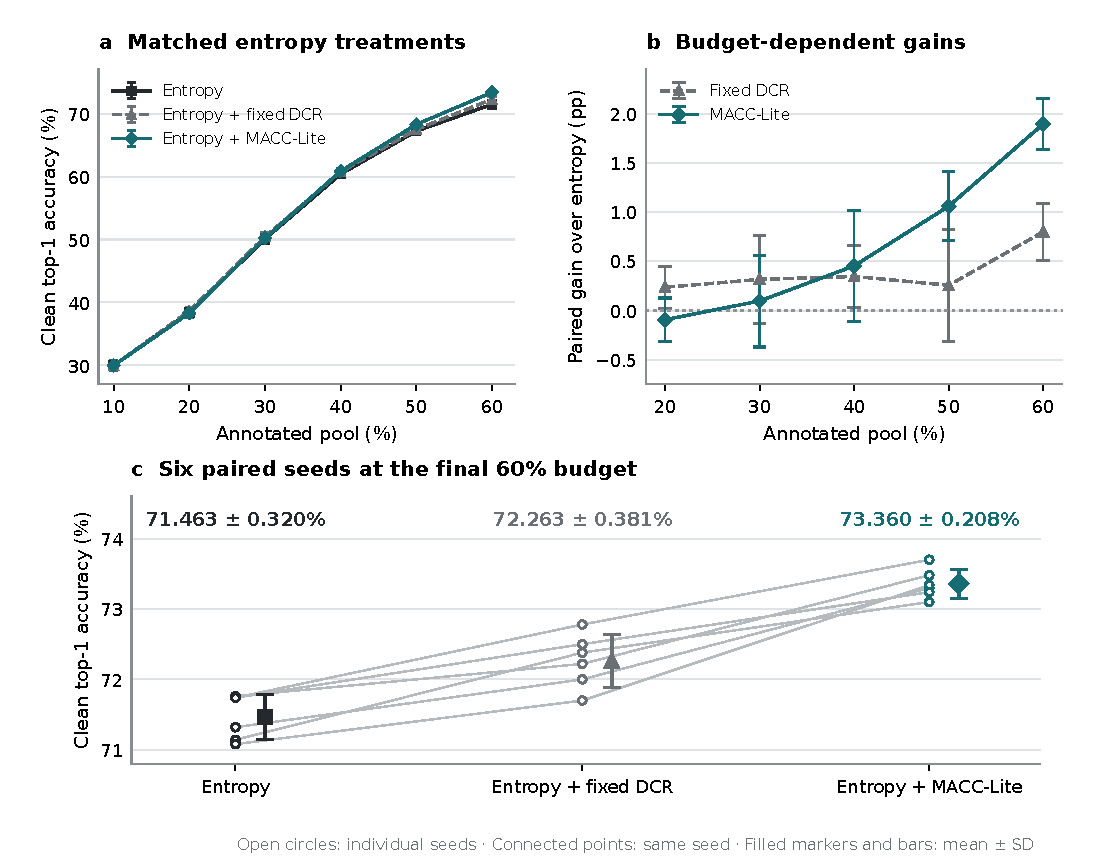
\includegraphics[width=\textwidth]{figures/figure4_entropy.pdf}
\caption{Matched entropy treatments across annotation budgets and seeds.
(a) Mean clean accuracy and sample SD across six seeds. (b) Mean and sample
SD of within-seed differences from entropy; the common 10\% initialization
has zero gain and is omitted. (c) Individual final-budget accuracies, with
lines joining the same seed across conditions; adjacent filled markers and
bars show mean $\pm$ sample SD. Overlapping seed values are retained.
These bars are not confidence intervals. Fixed DCR uses $\lambda_l=0.03$
and the same separation penalty as Lite. Lite is not uniformly better at
early budgets, but exceeds both comparators in all six final-budget seeds.
Only the final 60\% comparisons enter the declared follow-up tests. All
points derive from recorded measurements.}
\label{fig:entropy_budget}
\end{figure}

\begin{placedtable}
\caption{The later fixed-control study's two clean-accuracy contrasts.
Differences and individual unadjusted 95\% paired-$t$ intervals are in
percentage points. Holm correction is applied separately to the two
paired-$t$ and the two exact tests in this family. Prior families are unchanged.}
\label{tab:entropy_fixed_tests}
\centering\small
\begin{tabularx}{\textwidth}{@{}Yrrrrr@{}}
\toprule
Target minus reference & Difference & 95\% CI & Raw $t$ $p$ &
Adjusted $t$ $p$ & Exact raw / adjusted \\
\midrule
Entropy + fixed $-$ entropy & +0.800 & $[+0.498,+1.102]$ &
0.001047 & 0.001442 & 0.03125 / 0.0625 \\
Entropy + Lite $-$ entropy + fixed & +1.097 & $[+0.714,+1.479]$ &
0.000721 & 0.001442 & 0.03125 / 0.0625 \\
\bottomrule
\end{tabularx}
\end{placedtable}

\begin{multicols}{2}
\subsection{Comparison with UHerding-Margin}
\label{sec:uherding_results}

UHerding-Margin completes all five phases for each seed
and the full-set final evaluation.
Its mean clean accuracy is $71.747\pm0.626\%$,
versus $71.463\pm0.320\%$ for entropy and
$73.360\pm0.208\%$ for entropy with aligned DCR and Lite.
UHerding minus entropy is +0.283 points with
interval $[-0.430,+0.997]$, adjusted paired-$t$ value
0.3540, and adjusted exact value 0.3125.
This does not establish superiority or equivalence.

Entropy with the aligned Lite treatment exceeds the UHerding
adaptation in every seed. The mean difference is +1.613 points,
with interval $[+0.957,+2.270]$.
The adjusted paired-$t$ value is 0.002923;
the adjusted exact value is 0.0625.
This compares complete pipelines and does not establish
superiority of entropy alone, or of the combined treatment
over the authors' unmodified UHerding benchmark implementation.


UHerding retains one correct adversarial image for each of
seeds 802 and 805, and none otherwise:
mean robust accuracy $0.0067\%$.
The comparison adds an executed recent mechanism while retaining
its representation and selection-domain adaptations.
\end{multicols}

\begin{placedtable}
\caption{The UHerding comparison's two clean-accuracy contrasts,
in percentage points. Intervals are individual unadjusted 95\%
paired-$t$ intervals; each test column is Holm-adjusted
across these two comparisons only.}
\label{tab:uherding_tests}
\centering\small
\begin{tabularx}{\textwidth}{@{}Yrrrr@{}}
\toprule
Target minus reference & Difference & 95\% CI &
Adjusted $t$ $p$ & Adjusted exact $p$ \\
\midrule
UHerding-Margin $-$ entropy &
+0.283 & $[-0.430,+0.997]$ & 0.3540 & 0.3125 \\
Entropy + aligned Lite $-$ UHerding-Margin &
+1.613 & $[+0.957,+2.270]$ & 0.002923 & 0.0625 \\
\bottomrule
\end{tabularx}
\end{placedtable}

\begin{multicols}{2}
\subsection{Representation changes and learned-controller behavior}

Within the original matrix, geometry with aligned Lite has the
lowest mean log trace ratio, cross-entropy, and ECE.
Table~\ref{tab:geometry} reports descriptive geometry separately
from task performance. These statistics are not a causal
mediation analysis, and the all-class assessment ratio does not
establish attainment of the 16-class anchor target.

\end{multicols}

\begin{placedtable}
\caption{Final all-class normalized geometry, mean $\pm$ seed SD.
The statistic averages layer3 and layer4
$\log((W+\epsilon)/(B+\epsilon))$.}
\label{tab:geometry}
\centering\small
\begin{tabularx}{\linewidth}{@{}Yc@{}}
\toprule
Condition & Mean log trace ratio \\
\midrule
Random & $1.3881\pm0.0197$ \\
Entropy & $1.3916\pm0.0170$ \\
Acquisition only & $1.3864\pm0.0151$ \\
Random + aligned fixed & $1.0607\pm0.0218$ \\
\model{} + aligned fixed & $0.9767\pm0.0200$ \\
\model{} + aligned Lite & $0.4937\pm0.0390$ \\
\model{} + aligned Full & $1.0825\pm0.0982$ \\
Entropy + aligned fixed & $1.0027\pm0.0125$ \\
Entropy + aligned Lite & $0.4725\pm0.0434$ \\
\bottomrule
\end{tabularx}
\end{placedtable}

\begin{multicols}{2}
Full MACC executes 370, 368, 368, 374, 365, and 373
learned-policy updates for seeds 801--806.
Its mean accuracy is 0.237 points below aligned fixed DCR,
with an interval spanning zero, and 0.660 points below entropy.
The latter difference passes the adjusted paired-$t$ test.
The learned controller is active, but its additional capacity
does not establish benefit under the present settings.
Feedback horizon, changing acquisition phases, and imperfect
credit assignment are possible explanations rather than
identified causes.

Short development continuations found Lite coefficients below
the 0.10 cap. That observation does not substitute for a
long-run stability analysis.
Proposition~\ref{prop:bounded} bounds coefficients,
not the network's geometric state or task error.

\subsection{Adversarial robustness is not recovered}

Final checkpoints retain zero or one correct adversarial
prediction out of 5,000. Mean robust accuracy is approximately
$0.000\%$--$0.017\%$.
No planned robustness comparison establishes an improvement.
These near-zero empirical outcomes are not a population
certificate, and repeated predictions on the same images
do not become independent observations when pooled across seeds.

The original spectral pilot also had zero robustness at
$8/255$; extending its selected-checkpoint diagnostic from
1,000 to all 5,000 images reproduced that result.
Smaller-radius post-hoc diagnostics did not establish an
overall advantage over random acquisition.
The final study retains the original attack radius.
Improved clean performance and supervised geometry therefore
do not support the earlier robustness-benefit interpretation.

\subsection{C4: a small spectral-regularization effect}
\label{sec:c4_results}

Table~\ref{tab:c4_holdout} reports the unused local validation shard, and
Table~\ref{tab:c4_contrasts} gives all three NLL contrasts against baseline.
Fixed spectral DCR lowers NLL in every paired seed, with mean difference
$-0.00029250$ nats/token and individual interval
$[-0.00032813,-0.00025688]$. Its raw paired-$t$ value is
$4.42\times10^{-6}$ and its archived within-endpoint Holm-adjusted value is
$8.85\times10^{-6}$. The raw exact value is 0.03125; applying Holm
correction within the same three-contrast family gives 0.09375.

The effect is close to the original-shard difference of $-0.00028734$.
The second shard checks sensitivity to local data reuse but adds no
independent training seeds. The practical change is approximately
0.0086\% in NLL and 0.0292\% in perplexity. Fixed DCR does not establish a
token-accuracy or pooled-ECE benefit. Spectral Lite increases NLL in all
six seeds by a mean of $0.00194729$ nats/token, with interval
$[0.00187898,0.00201560]$. Full is inconclusive relative to baseline:
$+0.00023624$, interval $[-0.00018778,+0.00066025]$, raw paired-$t$ value
0.2115. This is not an equivalence result. The secondary comparison
outputs are retained in Appendix~\ref{app:c4_secondary}.
\end{multicols}

\begin{placedtable}
\caption{Unused-local-shard C4 evaluation of the same 24 final
GPT-2 checkpoints. Values are mean $\pm$ sample SD over six
training seeds, with 1,999,872 next-token predictions per checkpoint.
The formulations are spectral, not aligned classification DCR.}
\label{tab:c4_holdout}
\centering\small
\begin{tabularx}{\textwidth}{@{}Ycccc@{}}
\toprule
Condition & NLL (nats/token) & Perplexity &
Pooled token ECE & Token accuracy \\
\midrule
Baseline &
$3.384212\pm0.000239$ & $29.49473\pm0.00705$ &
$0.012324\pm0.000426$ & $0.380067\pm0.000123$ \\
Fixed spectral DCR &
$3.383919\pm0.000253$ & $29.48611\pm0.00746$ &
$0.012216\pm0.000438$ & $0.380029\pm0.000083$ \\
Spectral MACC-Lite &
$3.386159\pm0.000220$ & $29.55222\pm0.00651$ &
$0.013131\pm0.000396$ & $0.379920\pm0.000098$ \\
Spectral Full MACC &
$3.384448\pm0.000462$ & $29.50170\pm0.01362$ &
$0.012438\pm0.000584$ & $0.380040\pm0.000111$ \\
\bottomrule
\end{tabularx}
\end{placedtable}

\begin{placedtable}
\caption{All three unused-shard C4 NLL contrasts. Differences and individual
95\% paired-$t$ intervals are in $10^{-4}$ nats/token; negative differences
favor regularization. Holm adjustment is within the three NLL contrasts,
separately for each test. Both test families use the same three contrasts; intervals are unadjusted.}
\label{tab:c4_contrasts}
\centering\small
\begin{tabularx}{\textwidth}{@{}Yrrrrrr@{}}
\toprule
Condition minus baseline & Difference & 95\% CI &
Raw $t$ $p$ & Holm $t$ $p$ & Raw exact $p$ & Holm exact $p$ \\
\midrule
Fixed spectral DCR & $-2.92505$ & $[-3.28129,-2.56881]$ & $4.4239\times10^{-6}$ & $8.8477\times10^{-6}$ & 0.03125 & 0.09375 \\
Spectral MACC-Lite & $+19.47289$ & $[+18.78979,+20.15599]$ & $8.9651\times10^{-9}$ & $2.6895\times10^{-8}$ & 0.03125 & 0.09375 \\
Spectral Full MACC & $+2.36236$ & $[-1.87778,+6.60250]$ & 0.21152 & 0.21152 & 0.21875 & 0.21875 \\
\bottomrule
\end{tabularx}
\end{placedtable}

\begin{multicols}{2}
The language controller records 488 actions per seed.
Lite spends much of training at the 0.08 coefficient cap;
Full records 428--445 learned-policy updates.
The adaptive results therefore do not reflect an inactive
controller. Effective ranks increase under regularization,
so the mechanism is spectral shaping rather than uniformly
stronger low-rank collapse.
The small fixed-DCR NLL result does not establish broader
calibration, memorization, or cross-modal gains.

\subsection{Diffusion: fine-tuning helps, spectral regularization does not}
\label{sec:diffusion_results}

Unregularized fine-tuning lowers mean FID from 10.512 to 8.057.
Fixed spectral DCR, Lite, and Full instead increase FID
relative to that baseline by 0.156, 0.415, and 0.154.
Each increase occurs in every seed.
Improvement over the unchanged pretrained model therefore
does not establish added value from DCR.
\end{multicols}

\begin{placedtable}
\caption{Diffusion confirmation with 50,000 generated images per
condition and seed. Values are mean $\pm$ sample SD over six
seed streams. FID is primary. Reference variation is sampling
variation for one unchanged pretrained model.}
\label{tab:diffusion_final}
\centering\small
\begin{tabularx}{\textwidth}{@{}Yccc@{}}
\toprule
Condition & FID $\downarrow$ &
KID $\times10^3\downarrow$ & Inception score $\uparrow$ \\
\midrule
Pretrained reference &
$10.512\pm0.100$ & $9.153\pm0.124$ & $8.479\pm0.039$ \\
Unregularized fine-tuning &
$\mathbf{8.057\pm0.048}$ & $6.605\pm0.084$ & $8.692\pm0.043$ \\
Fixed spectral DCR &
$8.213\pm0.070$ & $6.726\pm0.105$ & $8.724\pm0.049$ \\
Spectral MACC-Lite &
$8.472\pm0.100$ & $6.939\pm0.115$ & $8.728\pm0.055$ \\
Spectral Full MACC &
$8.211\pm0.116$ & $6.744\pm0.088$ & $8.729\pm0.050$ \\
\bottomrule
\end{tabularx}
\end{placedtable}

\begin{placedtable}
\caption{All four diffusion FID contrasts.
Positive differences indicate worse FID for the target.
Intervals are individual unadjusted paired-$t$ intervals.
Each test family is Holm-adjusted over these four comparisons.}
\label{tab:diffusion_contrasts}
\centering\small
\begin{tabularx}{\textwidth}{@{}Yrrrr@{}}
\toprule
Target minus reference & Difference & 95\% interval &
Adjusted $t$ $p$ & Adjusted exact $p$ \\
\midrule
Baseline $-$ pretrained reference &
$-2.45468$ & $[-2.58346,-2.32589]$ &
$2.6769\times10^{-7}$ & 0.125 \\
Fixed DCR $-$ baseline &
+0.15601 & $[+0.11357,+0.19845]$ & 0.0004481 & 0.125 \\
MACC-Lite $-$ baseline &
+0.41472 & $[+0.31931,+0.51012]$ & 0.0003004 & 0.125 \\
Full MACC $-$ baseline &
+0.15431 & $[+0.06205,+0.24658]$ & 0.0077204 & 0.125 \\
\bottomrule
\end{tabularx}
\end{placedtable}

\begin{multicols}{2}
All four contrasts pass their adjusted paired-$t$ tests.
Each raw exact value is 0.03125, giving adjusted value 0.125.
The consistent adverse direction is retained with the
small-sample assumptions and resolution qualification.
It is not a claim that every diffusion regularizer is harmful.

KID is also higher in mean under every regularized condition.
Slightly higher Inception scores remain secondary and do not
replace FID.
Mean official-test EMA denoising MSE is 0.02918539 for baseline,
0.02918606 for fixed DCR, 0.02918634 for Lite, and
0.02918632 for Full, compared with 0.02935395 for the reference.
These small descriptive differences are not formal
equivalence or significant secondary effects.

Full executes 188, 186, 189, 185, 183, and 186 learned
updates, with 200 controller events per seed.
Lite also executes 200 events and ends at the 0.05 cap.
The final value does not specify its occupancy over training.
Final monitored ranks are approximately 23--24 for baseline,
49 for fixed DCR, 38--39 for Lite, and 42--60 for Full.
Active control and representation changes do not establish
target attainment or better generation.

The two-seed pilot favored fixed DCR and Full relative to its
baseline. That direction does not persist in confirmation.
Training horizon and generated-sample count both changed,
so the present comparison does not isolate the reason
for the reversal.

\subsection{Audio captioning: no established CIDEr-D improvement}
\label{sec:audio_results}

Fixed DCR has a slightly higher mean CIDEr-D than baseline;
Lite and Full have lower means.
Every primary interval spans zero, and both adjusted test
families give $p=1.0000$ for all three contrasts.
This is an inconclusive comparison, not proof of equivalence,
zero population effect, or universal ineffectiveness.
\end{multicols}

\begin{placedtable}
\caption{AudioCaps results on the fixed available subset:
mean $\pm$ sample SD over seeds 1301--1306.
Each run uses 866 test clips with five references each.
Metrics retain their native scales; CIDEr-D is primary.}
\label{tab:audio_final}
\centering\small
\begin{tabularx}{\textwidth}{@{}Yccccc@{}}
\toprule
Condition & CIDEr-D & BLEU-4 & METEOR & SPICE & SPIDEr \\
\midrule
Baseline &
$0.6736\pm0.0220$ & $0.2401\pm0.0137$ &
$0.2328\pm0.0043$ & $0.1664\pm0.0046$ & $0.4200\pm0.0132$ \\
Fixed spectral DCR &
$0.6745\pm0.0185$ & $0.2384\pm0.0114$ &
$0.2335\pm0.0022$ & $0.1650\pm0.0041$ & $0.4198\pm0.0110$ \\
Spectral MACC-Lite &
$0.6668\pm0.0212$ & $0.2378\pm0.0108$ &
$0.2320\pm0.0035$ & $0.1664\pm0.0020$ & $0.4166\pm0.0112$ \\
Spectral Full MACC &
$0.6703\pm0.0175$ & $0.2382\pm0.0094$ &
$0.2319\pm0.0023$ & $0.1659\pm0.0041$ & $0.4181\pm0.0100$ \\
\bottomrule
\end{tabularx}
\end{placedtable}

\begin{placedtable}
\caption{All three primary audio CIDEr-D contrasts.
Positive differences favor the target.
Intervals are individual unadjusted paired-$t$ intervals;
each test family is Holm-adjusted across three comparisons.}
\label{tab:audio_contrasts}
\centering\small
\begin{tabularx}{\textwidth}{@{}Yrrrr@{}}
\toprule
Target minus baseline & Difference & 95\% interval &
Adjusted $t$ $p$ & Adjusted exact $p$ \\
\midrule
Fixed spectral DCR &
+0.000896 & $[-0.016040,+0.017833]$ & 1.0000 & 1.0000 \\
Spectral MACC-Lite &
$-0.006781$ & $[-0.028950,+0.015389]$ & 1.0000 & 1.0000 \\
Spectral Full MACC &
$-0.003329$ & $[-0.015313,+0.008656]$ & 1.0000 & 1.0000 \\
\bottomrule
\end{tabularx}
\end{placedtable}

\begin{multicols}{2}
Seed-level CIDEr-D values are reported in Appendix~\ref{app:classification_details}.

Raw paired-$t$ values are 0.8971, 0.4673, and 0.5072;
raw exact values are 0.84375, 0.50000, and 0.53125.
Unlike a case resting only on the exact-test resolution limit,
these raw results also provide no strong evidence of a difference.
Mean test NLL is 2.026833 for baseline, 2.029867 for fixed,
2.033260 for Lite, and 2.030362 for Full.
These remain descriptive secondary results.

Full records 260, 253, 260, 266, 259, and 254 learned-policy
updates. Both adaptive conditions record 278 events.
All 24 runs produce 866 nonempty captions.
The mismatched-audio development diagnostic has higher NLL
than correctly paired audio in every run.
That establishes sensitivity to the supplied conditioning
under this diagnostic, not added benefit from DCR or
a comprehensive grounding guarantee.

The pilot evaluates 376 development clips after two epochs;
confirmation evaluates 866 test clips after ten epochs.
Their absolute scores cannot attribute a difference solely
to training duration.
The study evaluates audio--text captioning; audio retrieval, audio classification,
other architectures, and full-original-benchmark comparability
remain outside its scope.


\subsection{Computational cost and memory}
\label{sec:overhead}

Table~\ref{tab:compute} reports ImageNet-100 components.
The synchronized training-compute timer includes forward,
loss, backward, clipping, and optimizer execution, but excludes
subsequent controller observation and policy operations.
Feedback and acquisition have separate timers.
Loading, serialization, evaluation, and orchestration are not
fully represented by summing these columns.
All references record geometry, and initialization is allocated
once per conceptual condition.
\end{multicols}

\begin{placedtable}
\caption{Recorded ImageNet-100 timing components in seconds
per conceptual condition run, averaged over six seeds.
Training and feedback include their allocated shared-initialization
costs. These are component, not complete application, timings.}
\label{tab:compute}
\centering\small
\begin{tabularx}{\textwidth}{@{}Yrrrr@{}}
\toprule
Method & Training compute & Feedback inference &
Acquisition & Final AutoAttack \\
\midrule
Random & 5093.24 & 182.25 & 0.85 & 792.52 \\
Entropy & 5092.81 & 182.45 & 490.83 & 800.95 \\
BADGE & 5093.97 & 182.55 & 523.26 & 775.80 \\
Noise Stability & 5093.61 & 182.52 & 2942.89 & 777.36 \\
Acquisition only & 5093.23 & 182.38 & 739.69 & 798.50 \\
Random + aligned fixed & 5240.51 & 182.30 & 0.86 & 811.51 \\
\model{} + aligned fixed & 5238.40 & 182.28 & 740.18 & 820.73 \\
\model{} + aligned Lite & 5238.85 & 182.27 & 739.58 & 804.70 \\
\model{} + aligned Full & 5240.13 & 182.30 & 738.97 & 783.91 \\
\bottomrule
\end{tabularx}
\end{placedtable}

\begin{multicols}{2}
The maximum PyTorch-allocated memory is 6,075,090,432 bytes
for every conceptual run in the original nine-condition matrix.
Shared initialization may dominate that maximum;
equal values do not establish zero additional controller memory.
The phase-specific comparison below is narrower but still
does not isolate a complete controller footprint.
\end{multicols}

\begin{placedtable}
\caption{Post-initialization training time and peak allocation.
Duration is the mean sum over five post-initialization
training phases. Peaks describe PyTorch allocation in
those phases, not isolated controller memory.}
\label{tab:phase_cost}
\centering\small
\begin{tabularx}{\textwidth}{@{}Yrr@{}}
\toprule
Condition & Five-phase duration (s) & Recorded phase peak (bytes) \\
\midrule
Entropy & 5,255.02 & 6,066,439,680 \\
Entropy + aligned MACC-Lite & 5,391.31 & 6,066,701,824 \\
\midrule
Difference & +136.29 & +262,144 \\
\bottomrule
\end{tabularx}
\end{placedtable}

\begin{multicols}{2}
The duration in Table~\ref{tab:phase_cost} and the synchronized
training-compute component in Table~\ref{tab:compute} have different
measurement boundaries. The former is a phase-duration record; the
latter excludes controller observation and policy operations and includes
an allocated initialization component. They are not additive or directly
subtractable. These timers do not define a common end-to-end boundary.

The entropy-plus-Lite mean phase duration is 2.59\% higher,
a difference of 136.29 s. These are sequential campaigns,
not interleaved timing trials.
The peak difference is 262,144 bytes, or 0.25 MiB.
Neither quantity is complete application overhead or
an isolated controller measurement.


The entropy-plus-fixed follow-up separately records means of 4,837.85~s
for synchronized training compute, 182.55~s for feedback inference,
483.99~s for acquisition, and 782.66~s for final AutoAttack.
The training and feedback components exclude the reused initialization;
they therefore cannot be inserted directly into Table~\ref{tab:compute}
or compared as complete application time. The fixed-control records do not contain a phase-duration or phase-peak memory aggregate for this
new condition, so no new overhead ratio is inferred.

A five-pair GPT-2/C4 microbenchmark times 250 optimizer steps.
Plain execution takes $33.5293\pm0.0429$ s;
the sampled-monitoring path takes $33.7633\pm0.0731$ s.
The paired time increase is $0.698\%$ with SD 0.142
percentage points; peak allocation increases about 0.089 GiB.
Its BF16 parameters, microbatches of two sequences with
four accumulation passes, ten monitor events, optimizer
initialization, and timing boundary differ from production.

Production C4 time increases by 7.88\%, 7.68\%, and 16.62\%
for fixed, Lite, and Full relative to its monitored baseline.
These ratios cannot be combined with the microbenchmark
to obtain total overhead relative to plain training.

Diffusion mean task-job wall times are 1,616.81 s for
reference sampling and 2,919.80, 2,974.48, 2,978.48,
and 2,977.43 s for baseline, fixed, Lite, and Full.
They include task-driver training, sampling, and metrics,
but exclude the wrapper's later official-test EMA assessment
and study preparation. The reference has no training updates
and is not an overhead denominator.

Audio successful training-loop times span
1,175.53--1,201.80 s for baseline,
1,308.80--1,333.21 s for fixed,
1,309.24--1,337.74 s for Lite, and
1,336.39--1,375.73 s for Full.
These include controller feedback and checkpoints but exclude
setup, final decoding, metrics, and saved-result audits.
Feature extraction is reused from the pilot.
Rejected initialization attempts and verification are separate.
No universal sub-10\% or end-to-end overhead claim follows.
\end{multicols}
\begin{multicols}{2}
\section{Discussion and limitations}\label{sec:discussion}

\subsection{What objective alignment contributes}

The principal classification finding is a favorable
\emph{combined aligned-loss-and-Lite treatment} within the
evaluated training regime.
The original matrix supplies matched fixed-versus-none
and Lite-versus-fixed comparisons under geometric acquisition.
The acquisition-rule ablation supplies a favorable combined-treatment
comparison and shows that the geometry score is unnecessary
for the strongest observed mean.

The later entropy-plus-fixed control separates two observed treatment
contrasts: +0.800 points for adding the fixed aligned loss and safeguard,
and a further +1.097 points for replacing the fixed coefficient with
Lite. Their sum recovers the +1.897-point combined-treatment difference.
This arithmetic is a decomposition of matched pipeline contrasts, not a
causal mediation analysis of geometry, feedback, or selected examples.
The adaptive policy can also change subsequent acquired sets.

The fixed comparator uses $\lambda_l=0.03$. A broader claim for feedback
should address an independently tuned fixed strength or a prespecified
open-loop schedule with comparable tuning resources. The experiments
do not separately isolate normalization and the separation safeguard.
Attribution specifically to objective--feedback alignment would require
a controlled comparison that changes alignment while matching the
remaining optimization and sampling choices. The favorable final-budget
contrast should also be distinguished from the mixed early-budget
ordering in Figure~\ref{fig:entropy_budget}.

Full MACC receives feedback and updates its policy in every seed,
but its task outcomes are inconclusive or unfavorable.
Its outcome is conditional on the specified state, reward,
action, and horizon. A different controller might perform
differently, but the present results do not establish why
additional policy capacity fails to improve the task.

The UHerding comparison is similarly conditional on its
fixed shared-initial supervised features, capped candidate
passes, holdout temperature calibration, and warm-start
training. The combined entropy-plus-Lite result is not
a general rejection of uncertainty-weighted coverage.

Table~\ref{tab:claim_boundaries} summarizes the empirical scope.
\end{multicols}

\begin{placedtable}
\caption{Supported observations and claims not established.
These distinctions apply to the reported protocols rather
than all possible implementations of the framework.}
\label{tab:claim_boundaries}
\centering\small
\begin{tabularx}{\textwidth}{@{}p{0.23\textwidth}YY@{}}
\toprule
Question & Supported observation & Not established \\
\midrule
Classification alignment &
Loss and feedback share the supervised log trace ratio &
Necessity, global stability, or global optimality \\
Active learning &
Matched six-seed budget comparison and favorable component directions &
Universal superiority or equal-performance 40\% label savings \\
MACC-Lite &
Favorable Lite-versus-fixed contrasts under geometric and entropy acquisition &
Superiority to tuned fixed strengths or schedules, isolated alignment
causality, or necessary geometric acquisition \\
Full MACC &
Learned regularization control executes in all seeds &
A task benefit from extra controller capacity or learned query thresholds \\
Adversarial robustness &
Full-set standard AutoAttack at the specified radius &
Meaningful robustness gains, certification, or deployment safety \\
Language modeling &
Small fixed spectral-DCR loss reduction on an unused local shard &
An aligned-classification-objective effect or universal language gains \\
Diffusion &
All spectral conditions have higher FID than matched fine-tuning &
Universal generative benefit or a test of aligned classification DCR \\
Audio captioning &
Six-seed available-subset test comparison without established CIDEr-D gain &
Equivalence, full-original-benchmark comparability, or general audio gains \\
\bottomrule
\end{tabularx}
\end{placedtable}

\begin{multicols}{2}
\subsection{Limits of the classification and statistical evidence}

The visual study uses one backbone, one 100-class subset,
a class-balanced sampler, and frozen post-initialization
BatchNorm statistics.
Matching methods within this regime does not make it their
best possible training recipe.
Official validation images were used for reporting during
development; new seeds quantify initialization and split
variation, not transfer to an entirely untouched image benchmark.

Geometric atypicality may prioritize unhelpful examples.
Aggregate scatter can conceal a poorly separated class pair,
and coefficient bounds do not establish stable optimization.
Training anchors and all-class assessment also differ in
class support and transforms.
There is no demonstrated advantage at the specified
adversarial endpoint or evidence of deployment safety.

The exact-test nonrejections have the structural limitation
derived in Section~\ref{sec:statistics}.
The adjusted paired-$t$ findings remain conditional on their
small-sample assumptions.
Neither procedure removes the post-hoc chronology of the
additional comparisons or provides programme-wide multiplicity control.
We retain the original comparison families instead of
reorganizing them after observing the outcomes.

\subsection{Cross-task scope and generalization limits}
\label{sec:extensions}

C4 concerns a small effect on a locally selected single-shard
subset with pretrained GPT-2.
Its unused-shard evaluation does not establish absence
of pretraining overlap.
Its spectral result cannot be attributed to the different
aligned classification objective.

Diffusion evaluates one pretrained CIFAR-10 U-Net,
one sampler, and one training schedule.
Every spectral condition has worse FID than the matched
fine-tuning baseline. This does not test aligned
classification DCR on diffusion, a separately tuned
regularization family, or large-scale text-to-image generation.

Audio captioning is conditional on an approximately
89\%-coverage third-party subset.
Exact identity and waveform checks do not prove acoustic
authenticity or exclude every near-duplicate.
AST pretraining may overlap underlying recordings,
and four flagged zero training clips remain in the frozen
policy. The study provides neither full-original-benchmark
comparability nor broader audio-retrieval, classification,
or grounding guarantees.
Its inconclusive primary contrasts do not establish
statistical equivalence.

The completed protocols thus cover classification, language,
image generation, and audio captioning, but support no
universal cross-task gain.
ImageNet-1K and ViT performance remain unevaluated.
The initialization workaround also limits claims of
seed-only byte-identical reproduction, as documented in
Appendix~\ref{app:provenance}.

\subsection{Reproducibility and data availability}
\label{sec:reproducibility}

The retained record includes protocols, source snapshots,
environment versions, splits, annotation accounting,
controller histories, checkpoint digests, and evaluation
outputs. Historical outcomes are preserved rather than
overwritten by later variants.
Appendix~\ref{app:provenance} summarizes data provenance and
verification boundaries.

Code, experiment configurations, numeric result records, and statistical
reconstruction scripts are available at
\url{https://github.com/alqithami/CANL}.
The repository distinguishes the historical pipeline from the later aligned
classification and spectral-confirmation implementations. It includes the
manuscript source and a reproducible analysis entry point. Raw licensed
data and large model checkpoints are excluded. The initialization and
verification limits in Appendix~\ref{app:provenance} remain applicable;
source availability is not a claim of independently repeated training.

\section{Conclusion}\label{sec:conclusion}
Objective-aligned representation control improves classification in the
specified ImageNet-100 protocol. Entropy acquisition with aligned DCR and
MACC-Lite reaches $73.360\pm0.208\%$ accuracy at 60\% annotations and exceeds
matched fixed strength by 1.097 percentage points. This supports the tested
adaptive treatment; it does not establish superiority over tuned fixed
schedules or meaningful adversarial robustness. Full MACC adds no
established classification benefit. The separate spectral studies yield a
small C4 loss reduction, worse diffusion FID, and inconclusive audio effects.
Representation control should therefore be judged by task performance,
with its objective, feedback rule, computational cost, and evaluation scope
made explicit.

\section*{Funding}
This research received no external funding or in-kind support.

\section*{Declaration of competing interest}
The author declares no known competing financial interests or personal
relationships that could have appeared to influence the work reported
in this paper.

\section*{CRediT authorship contribution statement}
Saad Alqithami: Conceptualization, Methodology, Data curation,
Formal analysis, Investigation, Project administration, Resources,
Software, Validation, Visualization, Writing -- original draft,
Writing -- review and editing.
\end{multicols}
\medskip
\appendix

\section{Seed-level results and development studies}\label{app:classification_details}
Tables~\ref{tab:entropy_lite_seeds}, \ref{tab:uherding_seeds}, and
\ref{tab:audio_seeds} report the paired observations underlying the main
comparisons. The experimental units and statistical families are defined
in Section~\ref{sec:statistics}.


\begin{placedtable}
\caption{Matched entropy treatments at 60\% annotations. Clean accuracies
are percentages; differences are percentage points. Entropy and Lite are
reused completed results. Lite robust-correct counts use standard
AutoAttack $8/255$ on all 5,000 validation images. Fixed DCR has 0/5,000
robust-correct images in every seed.}
\label{tab:entropy_lite_seeds}
\centering\small
\begin{tabularx}{\linewidth}{@{}c*{6}{>{\centering\arraybackslash}X}@{}}
\toprule
Seed & Entropy & Entropy + fixed & Entropy + Lite & Fixed $-$ entropy &
Lite $-$ fixed & Lite robust correct \\
\midrule
801 & 71.14 & 72.38 & 73.10 & +1.24 & +0.72 & 0/5,000 \\
802 & 71.76 & 72.22 & 73.48 & +0.46 & +1.26 & 1/5,000 \\
803 & 71.32 & 72.00 & 73.30 & +0.68 & +1.30 & 0/5,000 \\
804 & 71.74 & 72.78 & 73.70 & +1.04 & +0.92 & 0/5,000 \\
805 & 71.08 & 71.70 & 73.34 & +0.62 & +1.64 & 0/5,000 \\
806 & 71.74 & 72.50 & 73.24 & +0.76 & +0.74 & 0/5,000 \\
\midrule
Mean & 71.463 & 72.263 & 73.360 & +0.800 & +1.097 & --- \\
Sample SD & 0.320 & 0.381 & 0.208 & 0.288 & 0.364 & --- \\
\bottomrule
\end{tabularx}
\end{placedtable}


\begin{placedtable}
\caption{Matched UHerding comparison at 60\% annotations.
Entropy references are reused completed results.
UHerding uses the fixed-initial-R50 adaptation of
Section~\ref{sec:uherding_setup}. Robust counts refer
to the new UHerding branches only.}
\label{tab:uherding_seeds}
\centering\small
\begin{tabularx}{\textwidth}{@{}YYYYY@{}}
\toprule
Seed & Entropy & UHerding-Margin & Entropy + aligned Lite &
UHerding robust correct \\
\midrule
801 & 71.14 & 71.58 & 73.10 & 0/5,000 \\
802 & 71.76 & 72.64 & 73.48 & 1/5,000 \\
803 & 71.32 & 72.38 & 73.30 & 0/5,000 \\
804 & 71.74 & 71.46 & 73.70 & 0/5,000 \\
805 & 71.08 & 71.40 & 73.34 & 1/5,000 \\
806 & 71.74 & 71.02 & 73.24 & 0/5,000 \\
\midrule
Mean $\pm$ SD & $71.463\pm0.320$ &
$71.747\pm0.626$ & $73.360\pm0.208$ & --- \\
\bottomrule
\end{tabularx}
\end{placedtable}

\begin{placedtable}
\caption{All six paired audio CIDEr-D values from the final
confirmation test evaluation.}
\label{tab:audio_seeds}
\centering\small
\begin{tabularx}{\linewidth}{@{}Yrrrr@{}}
\toprule
Seed & Baseline & Fixed & Lite & Full \\
\midrule
1301 & 0.699902 & 0.706662 & 0.695297 & 0.697474 \\
1302 & 0.683473 & 0.656485 & 0.683658 & 0.675072 \\
1303 & 0.634166 & 0.656615 & 0.658886 & 0.647493 \\
1304 & 0.681798 & 0.678712 & 0.663435 & 0.671009 \\
1305 & 0.672890 & 0.676179 & 0.633839 & 0.655220 \\
1306 & 0.669446 & 0.672400 & 0.665875 & 0.675435 \\
\bottomrule
\end{tabularx}
\end{placedtable}

\subsection{What the development studies established}

The aligned formulation was selected after a bounded mechanism
screen. Each source seed had a shared 200-step stabilization
and five matched 2,000-step continuations on a fixed labeled set.
The screen required a favorable geometric direction and an
assessment-loss increase no larger than 0.02 nats in either
seed. This was a development tolerance, not statistical
noninferiority.

Relative to no regularization, spectral DCR changed the
geometric-mean trace ratio by +0.077\% and +0.054\%.
Aligned fixed DCR changed it by $-2.009\%$ and $-2.365\%$;
aligned Lite by $-4.426\%$ and $-5.015\%$; and aligned
Full by $-1.691\%$ and $-1.300\%$.
Loss changes were mixed but within the screen's tolerance.
These findings motivated the subsequent end-to-end comparison;
they did not themselves establish annotation efficiency
or robustness.


\section{Data provenance and verification scope}\label{app:provenance}

The repository accompanying this paper records the dataset revisions,
source-file digests, experiment configurations, and exported per-seed
measurements. Classification uses the CMC ImageNet-100 class selection
from the original ImageNet images, preserved without reencoding.
The selected inventory contains 126,689 training and 5,000 validation
images. Locally recorded checksums establish consistency of these copies;
they are not independent upstream certification.

C4 training uses \path{en/c4-train.00000-of-01024.json.gz}; the controller
and development split uses \path{en/c4-validation.00000-of-00008.json.gz}.
The final holdout evaluation uses
\path{en/c4-validation.00002-of-00008.json.gz}.
The second shard was unused in local training and development; absence
of GPT-2 pretraining overlap is not established.

The original classification audit reconstructs metrics from saved
validation, feedback, and attack arrays. Subsequent report-level checks
reproduce the paired effects and statistical tests across classification,
C4, diffusion, and audio, including the entropy-treatment budget curves
and layer-geometry summaries. This verifies the arithmetic of exported
records. It does not independently regenerate predictions, adversarial
examples, generated images, or captions from raw inputs and checkpoints.
The server-recorded audio audits additionally reproduce caption metrics
from saved predictions and original references.

Audio initialization required a bounded retry for a pre-training
mismatch in the encoder positional parameter. A construction was accepted
only if its whole-model digest matched the original seed-specific record;
no training outcome or evaluation score entered that acceptance rule.
Completed outputs, seeds, and acceptance records were preserved. This
procedure enforces the recorded match but does not resolve the underlying
initialization nondeterminism. Accepted-state hashes alone cannot
reconstruct their tensors, and the availability of all corresponding
initial-state binaries is not established. Exact regeneration from seeds
alone is consequently not claimed.

Raw licensed images, corpus text, audio recordings, and large model
checkpoints are not distributed in the repository. Original data access
conditions and the audio subset's coverage and provenance limitations
continue to apply. The released code and numeric records permit statistical
reconstruction within these stated boundaries.

\section{Secondary C4 comparison statistics}\label{app:c4_secondary}
The unused-shard analysis reports three method--baseline
contrasts for each secondary endpoint. Table~\ref{tab:c4_secondary}
retains the effect estimates, individual intervals, and both raw tests,
with Holm correction within each endpoint. Its exact-adjustment column
is calculated from the archived raw exact values for consistent
presentation. Perplexity is descriptive rather than an independent
primary outcome. Positive differences are adverse for perplexity and ECE;
negative differences are adverse for token accuracy.

\begin{placedtable}
\caption{Complete secondary unused-shard C4 comparisons. Each panel has its
own three-contrast Holm family. Confidence intervals are individual and
unadjusted. The indicated scaling applies to both differences and intervals;
token ECE and token accuracy are proportions, not percentages.}
\label{tab:c4_secondary}
\centering\small
\begin{tabularx}{\textwidth}{@{}Yrrrrrr@{}}
\toprule
Condition minus baseline & Difference & 95\% CI &
Raw $t$ $p$ & Holm $t$ $p$ & Raw exact $p$ & Holm exact $p$ \\
\midrule
\multicolumn{7}{@{}l}{\emph{Perplexity: differences in $10^{-2}$}} \\
Fixed spectral DCR & $-0.86260$ & $[-0.96757,-0.75763]$ & $4.4061\times10^{-6}$ & $8.8122\times10^{-6}$ & 0.03125 & 0.09375 \\
Spectral MACC-Lite & $+5.74906$ & $[+5.54778,+5.95034]$ & $8.8781\times10^{-9}$ & $2.6634\times10^{-8}$ & 0.03125 & 0.09375 \\
Spectral Full MACC & $+0.69705$ & $[-0.55390,+1.94800]$ & 0.21147 & 0.21147 & 0.21875 & 0.21875 \\
\midrule
\multicolumn{7}{@{}l}{\emph{Pooled token ECE: differences in $10^{-4}$}} \\
Fixed spectral DCR & $-1.07333$ & $[-4.14827,+2.00161]$ & 0.41069 & 0.78043 & 0.37500 & 0.68750 \\
Spectral MACC-Lite & $+8.07857$ & $[+6.41836,+9.73877]$ & $5.7942\times10^{-5}$ & 0.00017 & 0.03125 & 0.09375 \\
Spectral Full MACC & $+1.14058$ & $[-1.97737,+4.25853]$ & 0.39021 & 0.78043 & 0.34375 & 0.68750 \\
\midrule
\multicolumn{7}{@{}l}{\emph{Token accuracy: differences in $10^{-4}$}} \\
Fixed spectral DCR & $-0.38336$ & $[-1.21617,+0.44945]$ & 0.28989 & 0.28989 & 0.28125 & 0.28125 \\
Spectral MACC-Lite & $-1.47509$ & $[-1.89933,-1.05086]$ & 0.00029 & 0.00088 & 0.03125 & 0.09375 \\
Spectral Full MACC & $-0.26752$ & $[-0.63924,+0.10420]$ & 0.12355 & 0.2471 & 0.09375 & 0.18750 \\

\bottomrule
\end{tabularx}
\end{placedtable}


% Flush every appendix float before the bibliography.

\begingroup
\small
\begin{multicols}{2}

\section*{Declaration of generative AI and AI-assisted technologies
in the manuscript preparation process}
ChatGPT (OpenAI) was used to assist with manuscript organization and
editing, mathematical exposition, programming and debugging,
interpretation of saved experimental artifacts, reference checking,
and preparation of the LaTeX figures. Research-process uses and
verification limits are described in Section~\ref{sec:computational_assistance}
and Appendix~\ref{app:provenance}.
The author is responsible for the scientific design, interpretation,
and content of this work.

\begin{thebibliography}{99}

\bibitem{papyan2020prevalence}
V. Papyan, X. Y. Han, D. L. Donoho,
Prevalence of neural collapse during the terminal phase of
deep learning training,
\emph{Proceedings of the National Academy of Sciences}
117(40) (2020) 24652--24663.
\doi{10.1073/pnas.2015509117}


\bibitem{settles2009active}
B. Settles,
\emph{Active Learning Literature Survey},
Computer Sciences Technical Report 1648,
University of Wisconsin--Madison, 2009; updated 26 January 2010.
\url{https://burrsettles.com/pub/settles.activelearning.pdf}


\bibitem{sener2018active}
O. Sener, S. Savarese,
Active learning for convolutional neural networks:
A core-set approach,
in: \emph{International Conference on Learning Representations}, 2018.
\url{https://arxiv.org/abs/1708.00489}


\bibitem{ash2020badge}
J. T. Ash, C. Zhang, A. Krishnamurthy, J. Langford, A. Agarwal,
Deep batch active learning by diverse, uncertain gradient lower bounds,
in: \emph{International Conference on Learning Representations}, 2020.
\url{https://openreview.net/forum?id=ryghZJBKPS}


\bibitem{fisher1936}
R. A. Fisher,
The use of multiple measurements in taxonomic problems,
\emph{Annals of Eugenics} 7 (1936) 179--188.
\doi{10.1111/j.1469-1809.1936.tb02137.x}


\bibitem{wen2016center}
Y. Wen, K. Zhang, Z. Li, Y. Qiao,
A discriminative feature learning approach for deep face recognition,
in: \emph{European Conference on Computer Vision}, 2016, pp. 499--515.
\doi{10.1007/978-3-319-46478-7_31}


\bibitem{dorfer2016deeplda}
M. Dorfer, R. Kelz, G. Widmer,
Deep linear discriminant analysis,
in: \emph{International Conference on Learning Representations}, 2016.
\url{https://arxiv.org/abs/1511.04707}


\bibitem{wang2026alignment}
J. Wang, Z. Gao, Z. Xie,
Space alignment matters: The missing piece for inducing
neural collapse in long-tailed learning,
\emph{Proceedings of the AAAI Conference on Artificial Intelligence}
40(31) (2026) 26302--26309.
\doi{10.1609/aaai.v40i31.39835}


\bibitem{alcala2026orthoplex}
J. Alcala, R. Andreeva, V. A. Kobzar, D. G. Mixon,
S. Na, S. Sule, Y. Xie,
Neural collapse in the orthoplex regime,
arXiv preprint arXiv:2603.20587, 2026.
\url{https://arxiv.org/abs/2603.20587}


\bibitem{li2024noise}
X. Li, P. Yang, Y. Gu, X. Zhan, T. Wang, M. Xu, C. Xu,
Deep active learning with noise stability,
\emph{Proceedings of the AAAI Conference on Artificial Intelligence}
38(12) (2024) 13655--13663.
\doi{10.1609/aaai.v38i12.29270}


\bibitem{jung2026aggregation}
C. Jung, S. Salehi, A. Schmeink,
Active learning using aggregated acquisition functions:
Accuracy and sustainability analysis,
\emph{IEEE Journal on Selected Topics in Signal Processing}, 2026.
\doi{10.1109/JSTSP.2026.3673105}
Author version: \url{https://arxiv.org/abs/2602.07440}


\bibitem{cui2026trustset}
G. Cui, Y. Liu, P. Wang, H. Hsu, X. Sun, X. Hao, Z. Liu,
Labeled TrustSet guided: Batch active learning with reinforcement learning,
in: \emph{International Joint Conference on Neural Networks}, 2026,
author manuscript.
\url{https://arxiv.org/abs/2604.12303}


\bibitem{bae2025uncertainty}
W. Bae, D. J. Sutherland, G. L. Oliveira,
Uncertainty herding: One active learning method for all label budgets,
in: \emph{International Conference on Learning Representations}, 2025.
\href{https://proceedings.iclr.cc/paper_files/paper/2025/hash/0302fb83c62991efbccf0a003e4f5a92-Abstract-Conference.html}
{ICLR 2025 proceedings}.


\bibitem{croce2020autoattack}
F. Croce, M. Hein,
Reliable evaluation of adversarial robustness with an ensemble
of diverse parameter-free attacks,
in: \emph{Proceedings of the 37th International Conference
on Machine Learning}, PMLR 119, 2020, pp. 2206--2216.
\url{https://proceedings.mlr.press/v119/croce20b.html}


\bibitem{guo2017calibration}
C. Guo, G. Pleiss, Y. Sun, K. Q. Weinberger,
On calibration of modern neural networks,
in: \emph{Proceedings of the 34th International Conference
on Machine Learning}, PMLR 70, 2017, pp. 1321--1330.
\url{https://proceedings.mlr.press/v70/guo17a.html}


\bibitem{williams1992}
R. J. Williams,
Simple statistical gradient-following algorithms
for connectionist reinforcement learning,
\emph{Machine Learning} 8 (1992) 229--256.
\doi{10.1007/BF00992696}


\bibitem{tian2020cmc}
Y. Tian, D. Krishnan, P. Isola,
Contrastive multiview coding,
in: \emph{European Conference on Computer Vision},
2020, pp. 776--794.
\doi{10.1007/978-3-030-58621-8_45}


\bibitem{deng2009imagenet}
J. Deng, W. Dong, R. Socher, L.-J. Li, K. Li, L. Fei-Fei,
ImageNet: A large-scale hierarchical image database,
in: \emph{IEEE Conference on Computer Vision and Pattern Recognition},
2009, pp. 248--255.
\doi{10.1109/CVPR.2009.5206848}


\bibitem{he2016deep}
K. He, X. Zhang, S. Ren, J. Sun,
Deep residual learning for image recognition,
in: \emph{IEEE Conference on Computer Vision and Pattern Recognition},
2016, pp. 770--778.
\doi{10.1109/CVPR.2016.90}


\bibitem{holm1979}
S. Holm,
A simple sequentially rejective multiple test procedure,
\emph{Scandinavian Journal of Statistics}
6(2) (1979) 65--70.
\url{https://www.jstor.org/stable/4615733}


\bibitem{radford2019gpt2}
A. Radford, J. Wu, R. Child, D. Luan, D. Amodei, I. Sutskever,
\emph{Language Models are Unsupervised Multitask Learners},
OpenAI technical report, 2019.
\href{https://cdn.openai.com/better-language-models/language_models_are_unsupervised_multitask_learners.pdf}
{Technical report}.


\bibitem{raffel2020}
C. Raffel, N. Shazeer, A. Roberts, K. Lee, S. Narang,
M. Matena, Y. Zhou, W. Li, P. J. Liu,
Exploring the limits of transfer learning with a
unified text-to-text transformer,
\emph{Journal of Machine Learning Research}
21(140) (2020) 1--67.
\url{https://jmlr.org/papers/v21/20-074.html}


\bibitem{ho2020denoising}
J. Ho, A. N. Jain, P. Abbeel,
Denoising diffusion probabilistic models,
in: \emph{Advances in Neural Information Processing Systems}
33, 2020, pp. 6840--6851.
\url{https://arxiv.org/abs/2006.11239}


\bibitem{krizhevsky2009cifar}
A. Krizhevsky,
\emph{Learning Multiple Layers of Features from Tiny Images},
technical report, University of Toronto, 2009.
\url{https://www.cs.toronto.edu/~kriz/cifar.html}


\bibitem{song2021ddim}
J. Song, C. Meng, S. Ermon,
Denoising diffusion implicit models,
in: \emph{International Conference on Learning Representations}, 2021.
\url{https://arxiv.org/abs/2010.02502}


\bibitem{heusel2017fid}
M. Heusel, H. Ramsauer, T. Unterthiner, B. Nessler, S. Hochreiter,
GANs trained by a two time-scale update rule converge
to a local Nash equilibrium,
in: \emph{Advances in Neural Information Processing Systems}
30, 2017.
\url{https://arxiv.org/abs/1706.08500}


\bibitem{binkowski2018mmd}
M. Bi\'nkowski, D. J. Sutherland, M. Arbel, A. Gretton,
Demystifying MMD GANs,
in: \emph{International Conference on Learning Representations}, 2018.
\url{https://arxiv.org/abs/1801.01401}


\bibitem{salimans2016gan}
T. Salimans, I. Goodfellow, W. Zaremba, V. Cheung,
A. Radford, X. Chen,
Improved techniques for training GANs,
in: \emph{Advances in Neural Information Processing Systems}
29, 2016.
\url{https://arxiv.org/abs/1606.03498}


\bibitem{kim2019audiocaps}
C. D. Kim, B. Kim, H. Lee, G. Kim,
AudioCaps: Generating captions for audios in the wild,
in: \emph{Proceedings of NAACL-HLT}, 2019, pp. 119--132.
\doi{10.18653/v1/N19-1011}


\bibitem{gong2021ast}
Y. Gong, Y.-A. Chung, J. Glass,
AST: Audio Spectrogram Transformer,
in: \emph{Interspeech}, 2021, pp. 571--575.
\doi{10.21437/Interspeech.2021-698}
\url{https://www.isca-archive.org/interspeech_2021/gong21b_interspeech.html}


\bibitem{gemmeke2017audioset}
J. F. Gemmeke, D. P. W. Ellis, D. Freedman, A. Jansen,
W. Lawrence, R. C. Moore, M. Plakal, M. Ritter,
Audio Set: An ontology and human-labeled dataset for audio events,
in: \emph{IEEE International Conference on Acoustics,
Speech and Signal Processing}, 2017.
\href{https://research.google/pubs/audio-set-an-ontology-and-human-labeled-dataset-for-audio-events/}
{Author publication record}.


\bibitem{vedantam2015cider}
R. Vedantam, C. L. Zitnick, D. Parikh,
CIDEr: Consensus-based image description evaluation,
in: \emph{IEEE Conference on Computer Vision and Pattern Recognition},
2015, pp. 4566--4575.
\href{https://openaccess.thecvf.com/content_cvpr_2015/html/Vedantam_CIDEr_Consensus-Based_Image_2015_CVPR_paper.html}
{CVPR open-access paper}.


\bibitem{papineni2002bleu}
K. Papineni, S. Roukos, T. Ward, W.-J. Zhu,
Bleu: A method for automatic evaluation of machine translation,
in: \emph{Proceedings of the 40th Annual Meeting of the
Association for Computational Linguistics}, 2002, pp. 311--318.
\doi{10.3115/1073083.1073135}


\bibitem{lin2004rouge}
C.-Y. Lin,
ROUGE: A package for automatic evaluation of summaries,
in: \emph{Text Summarization Branches Out}, 2004, pp. 74--81.
\url{https://aclanthology.org/W04-1013/}


\bibitem{denkowski2014meteor}
M. Denkowski, A. Lavie,
Meteor Universal: Language specific translation evaluation
for any target language,
in: \emph{Proceedings of the Ninth Workshop on Statistical
Machine Translation}, 2014, pp. 376--380.
\doi{10.3115/v1/W14-3348}


\bibitem{anderson2016spice}
P. Anderson, B. Fernando, M. Johnson, S. Gould,
SPICE: Semantic propositional image caption evaluation,
in: \emph{European Conference on Computer Vision}, 2016, pp. 382--398.
\doi{10.1007/978-3-319-46454-1_24}


\bibitem{liu2017spider}
S. Liu, Z. Zhu, N. Ye, S. Guadarrama, K. Murphy,
Improved image captioning via policy gradient optimization of SPIDEr,
in: \emph{IEEE International Conference on Computer Vision},
2017, pp. 873--881.
\href{https://openaccess.thecvf.com/content_iccv_2017/html/Liu_Improved_Image_Captioning_ICCV_2017_paper.html}
{ICCV open-access paper}.


\end{thebibliography}
\end{multicols}
\endgroup


\end{document}
